\documentclass[aspectratio=169, 10pt]{beamer}

%%%%%%%%%%%%%%%%%%%
% Beamer settings %
%%%%%%%%%%%%%%%%%%%
\usefonttheme{serif}
\setbeamertemplate{footline}[frame number]{}
\setbeamertemplate{navigation symbols}{}
\setbeamertemplate{items}[circle]
\setbeamertemplate{section in toc}[sections numbered]
\setbeamertemplate{frametitle continuation}{}
\setbeamertemplate{caption}[numbered]
\setbeamertemplate{section in toc shaded}[default][100]
\setbeamertemplate{enumerate items}[default]
\setbeamerfont{section in toc shaded}{series=\mdseries}
\setbeamerfont{section in toc}{series=\bfseries}

%%%%%%%%%%
% Images %
%%%%%%%%%%
\usepackage{graphicx}

%%%%%%%%%%
% Tables %
%%%%%%%%%%
\usepackage{booktabs}
\usepackage{multirow}

%%%%%%%%%%%%%%%%%%
% Math: Pacakges %
%%%%%%%%%%%%%%%%%%
\usepackage{amsmath}
\usepackage{amsfonts}
\usepackage{amssymb}
\usepackage{amsthm}
\usepackage{bm}
\usepackage{mathrsfs}

%%%%%%%%%%%%%%%%%%%%%%%%%%%%%%
% Math: Theorem Environments %
%%%%%%%%%%%%%%%%%%%%%%%%%%%%%%
\setbeamertemplate{theorems}[numbered]

\theoremstyle{definition}
\newtheorem{defn}{Definition}
\newtheorem*{defn*}{Definition}
\newtheorem{asm}{Assumption}
\newtheorem*{asm*}{Assumption}

\theoremstyle{plain}
\newtheorem{thm}{Theorem}
\newtheorem{lem}{Theorem}
\newtheorem{cor}{Corollary}
\newtheorem*{thm*}{Theorem}
\newtheorem*{lem*}{Lemma}
\newtheorem*{cor*}{Corollary}
\newtheorem*{prop*}{Proposition}

%%%%%%%%%%%%%%%%%%%%%%%%%%%%%%%
% Math: Operators and Symbols %
%%%%%%%%%%%%%%%%%%%%%%%%%%%%%%%
% Does not imply
% Source - https://tex.stackexchange.com/a/509385
% Posted by jds
% Retrieved 2026-03-30, License - CC BY-SA 4.0
\newcommand{\notimplies}{\;\not\mspace{-12mu}\implies}

% Independence in Probability Theory and Statistics.
\newcommand{\indep}{\mathrel{\perp\mspace{-11mu}\perp}}

% Indicators
\def\ind{\mathbf{1}}

% Probability operators
\def\Pr{\mathrm{Pr}}
\def\E{\mathrm{E}}
\def\Var{\mathrm{Var}}
\def\Cov{\mathrm{Cov}}
\def\Supp{\mathrm{support}}
\def\pto{\overset{\mathrm{p}}{\to}}
\def\dto{\rightsquigarrow}
\def\Normal{\mathrm{N}} % Normal distribution
\def\Unif{\mathrm{Uniform}} % Normal distribution

\def\Op{O_{\mathrm{p}}}
\def\op{o_{\mathrm{p}}}

% IID
\def\iid{\mathrm{iid}}

% Convenience for the paper
\def\FNA{\mathrm{FNA}}
\def\BA{\mathrm{BA}}
\def\INA{\mathrm{INA}}
\def\calL{\mathcal{L}}
\def\calF{\mathcal{F}}


\newcommand\mapsfrom{\mathrel{\reflectbox{\ensuremath{\mapsto}}}}

\usepackage[
authordate,backend=biber,natbib,maxcitenames=2
]{biblatex-chicago}

\addbibresource{2026-dae-smallpilots.bib}

\title{On the performance of the Neyman Allocation with small pilots}

\author{%
  \texorpdfstring{%
    \begin{columns}
      \column{.5\linewidth}
      \centering
      Yong Cai \\ University of Wisconsin
      \column{.5\linewidth}
      \centering
      Ahnaf Rafi \\ University of Virginia
    \end{columns}
 }
 {Yong Cai (UW-Madison), Ahnaf Rafi (UVA)}
}

\date{%
Design and Analysis of Experiments, Rutgers University \\
\hfill \\
May 2026}

\begin{document}

\begin{frame}[plain,noframenumbering]
\titlepage
\end{frame}

%%%%%%%%%%%%%%%%%%%%%%%%%%%%%%%%%%%%%%%%%%%%%%%%%%%%%%%%%%%%%%%%%%%%%%%%%%%%%%%%
\section*{Introduction}
%%%%%%%%%%%%%%%%%%%%%%%%%%%%%%%%%%%%%%%%%%%%%%%%%%%%%%%%%%%%%%%%%%%%%%%%%%%%%%%%

\begin{frame}
\frametitle{Motivation: two-wave experiments}
\begin{itemize}
  \item Improved estimation precision is often an objective in experimental
    design.
    \vfill
  \item A recent literature explores ways to do this in two-wave experiments:
    \vfill
    \begin{itemize}
      \item \textbf{Wave 1 (pilot):} smaller scale; used to check feasibility of
        experiment and improve main experiment wave.
        \vfill
      \item \textbf{Wave 2:} large main, used to estimate the ATE.
    \end{itemize}
    \vfill
  \item How to improve precision in main wave?
    \vfill
    \begin{itemize}
      \item Choose optimal treatment proportions ---
        \textbf{the Neyman Allocation} \citep{1934neymanTwoDifferentAspects}.
        \vfill
      \item Choose good ways to use additional covariates if you have them.
    \end{itemize}
    \vfill
  \item We focus on implementation issues for the first problem here.
    \vfill
    \begin{itemize}
      \item \textbf{Motivation:} most experiments running pilots in economics
        few experimental subjects (\(\leq 20\)).
        typically have 20 subjects or fewer.
    \end{itemize}
\end{itemize}
\end{frame}

%%%%%%%%%%%%%%%%%%%%%%%%%%%%%%%%%%%%%%%%%%%%%%%%%%%%%%%%%%%%%%%%%%%%%%%%%%%%%%%%
\section{Setup}
%%%%%%%%%%%%%%%%%%%%%%%%%%%%%%%%%%%%%%%%%%%%%%%%%%%%%%%%%%%%%%%%%%%%%%%%%%%%%%%%

\begin{frame}[plain,noframenumbering]
  \frametitle{Outline}
  \tableofcontents[currentsection]
\end{frame}

\begin{frame}
\frametitle{Setup}

\begin{itemize}
  \item Binary treatment. \emph{Potential outcomes:}
    \((Y (0), Y (1)) \sim F\) [infinite superpopulation].
    \emph{Observed outcome:} \(Y = A Y (1) + (1 - A) Y (0)\) for treatment
    assignment \(A\).
    \vfill
  \item Two waves:
    \vfill
    \begin{itemize}
      \item \textbf{Pilot:} \(m\) i.i.d.\ draws \(\{\tilde{Y}_{j} (0),
        \tilde{Y}_{j} (1)\}\).
        \vfill
      \item \textbf{Main wave:} \(n\) further i.i.d.\ draws, \(\{Y_{i} (0),
        Y_{i} (1)\}\) independent of pilot.
    \end{itemize}
    \vfill
  \item Researcher assigns treatments \(\tilde{A}_{i}\) and \(A_{i}\) (pilot and
    main resp.) s.t.
    \vfill
    \begin{itemize}
      \item 50-50 complete randomization in pilot wave with \(\{\tilde{A}_{i}\}
        \indep \{\tilde{Y}_{i} (0), \tilde{Y}_{i} (1)\}\),
        \vfill
      \item Main wave randomization maintains exogeneity/ignorability:
        \begin{equation*}
          \{Y_{i} (0), Y_{i} (1)\} \indep (\{A_{i}\}, \{\tilde{Y}_{j} (0),
          \tilde{Y}_{j} (1), \tilde{A}_{j}\}).
        \end{equation*}
        Main wave assignments also completely randomized, but can use
        information from pilot.
    \end{itemize}
\end{itemize}
\end{frame}

\begin{frame}
\frametitle{Estimation of ATE and the Neyman Allocation}
\begin{itemize}
  \item \emph{Target parameter:} \(\theta = \E[Y(1) - Y(0)]\), estimated by
     difference in treatment arm means
    \begin{equation*}
      \hat{\theta} = \frac{\sum_{i = 1}^{n} A_{i} Y_{i}}{\sum_{i = 1}^{n} A_{i}}
      - \frac{\sum_{i = 1}^{n} (1 - A_{i}) Y_{i}}{\sum_{i = 1}^{n} (1 - A_{i})}.
    \end{equation*}
    \vfill
  \item If \(\bar{A} = \frac{1}{n} \sum_{i = 1}^{n} A_{i} \pto \pi\), then
    \(\sqrt{n} (\hat{\theta} - \theta) \dto \Normal \left( 0, \frac{\sigma^{2}
      (1)}{\pi} + \frac{\sigma^{2} (0)}{1 - \pi} \right)\); \(\sigma^{2} (a) =
    \Var [Y (a)]\).
    \vfill
  \item \textbf{Neyman allocation:} choose \(\pi_{\ast}\) to minimize asymptotic
    variance:
    \begin{equation*}
      \pi_{\ast} = \frac{\sigma (1)}{\sigma (1) + \sigma (0)}
      \qquad
      \left[
      \implies
      \text{optimal variance} = (\sigma (1) + \sigma (0))^{2} \right].
    \end{equation*}
    \vfill
    \begin{itemize}
      \item \textbf{Intuition:} assign higher proportion to arm that is more
        difficult to learn about.
        \vfill
      \item \textbf{Note:} \(\pi_{\ast} = 1/2\) if \(\sigma (1) = \sigma (0)\).
    \end{itemize}
    \vfill
  \item Infeasible: \(\sigma^{2} (a)\) are unknown.
\end{itemize}
\end{frame}

\begin{frame}
\frametitle{The Feasible Neyman Allocation (FNA)}
\begin{itemize}
  \item Form estimate \(\tilde{\sigma}_{m}^{2} (a)\) of
    \(\sigma^{2} (a)\) from pilot and plug in: \(\tilde{\pi} =
    \frac{\tilde{\sigma}_{m} (1)}{\tilde{\sigma}_{m} (1) + \tilde{\sigma}_{m}
    (0)}\).
    \vfill
  \item Can use sample treatment group variances (or Bessel-corrected
    counterpart):
    \begin{equation*}
      \tilde{\sigma}_{m}^{2} (a) = \frac{\sum_{j = 1}^{m} \ind \{\tilde{A}_{j} =
      a\} \tilde{Y}_{j}^{2}}{\sum_{j = 1}^{m} \ind \{\tilde{A}_{j} = a\}} -
      \left( \frac{\sum_{j = 1}^{m} \ind \{\tilde{A}_{j} = a\}
      \tilde{Y}_{j}}{\sum_{j = 1}^{m} \ind \{\tilde{A}_{j} = a\}} \right)^{2}.
    \end{equation*}
    \vfill
  \item If \(\tilde{\sigma}_{m}^{2} (a) \pto \sigma^{2} (a)\) as \(m \to
    \infty\), then as \(\min \{m, n\} \to \infty\), (see
    e.g. \citet{2011hahnAdaptiveExperimentalDesign})
    \begin{equation*}
      \sqrt{n} (\hat{\theta} - \theta) \dto \Normal \left( 0, \frac{\sigma^{2}
      (1)}{\pi_{\ast}} + \frac{\sigma^{2} (0)}{1 - \pi_{\ast}} \right) =
      \Normal (0, (\sigma (1) + \sigma (0))^{2}).
    \end{equation*}
    \vfill
  \item If pilot is large, \(\hat{\theta}\) with FNA has asymptotic efficiency
    equal to infeasible NA.
\end{itemize}
\end{frame}

\begin{frame}
\frametitle{Allocation schemes for comparison}
Assume main wave assignments are chosen to ensure exactly \(\lfloor n \pi
\rfloor\) treated for \(\pi \in (0, 1)\).

\vfill

Consider three possible \(\pi\)'s:
\vfill
\begin{itemize}
  \item \emph{Infeasible Neyman Allocation (INA):}
    \(\pi_{*} = \dfrac{\sigma(1)}{\sigma(1) + \sigma(0)}\).
    \vfill
  \item \emph{Feasible Neyman Allocation (FNA):}
    \(\tilde{\pi} = \frac{\tilde\sigma_m(1)}{\tilde\sigma_m(1) +
    \tilde\sigma_m(0)}\).
    \vfill
  \item \emph{Balanced Allocation (BA):} \(\pi = 1/2\).
\end{itemize}
\vfill
By definition INA is best; for large \(m\) \(\FNA \approx \mathrm{INA}\).
Questions for \textbf{fixed} \(m\):
\vfill
\begin{enumerate}
  \item How does FNA behave as \(n \to \infty\)?
    \vfill
  \item Can BA beat FNA and if so, when?
\end{enumerate}
\end{frame}

%%%%%%%%%%%%%%%%%%%%%%%%%%%%%%%%%%%%%%%%%%%%%%%%%%%%%%%%%%%%%%%%%%%%%%%%%%%%%%%%
\section{Theoretical results}
%%%%%%%%%%%%%%%%%%%%%%%%%%%%%%%%%%%%%%%%%%%%%%%%%%%%%%%%%%%%%%%%%%%%%%%%%%%%%%%%

\begin{frame}
\frametitle{Asymptotics}
\begin{prop*}
Under FNA, with \(m\) fixed and \(n \to \infty\),
\begin{equation*}
  \sqrt{n} (\hat{\theta} - \theta)
  \dto \mathcal{L}_{m}, \quad \text{where} \quad
  \Pr(\mathcal{L}_m \le t) = \int_{0}^{1} \Phi \left( t / s (\pi) \right)
  G_{m} (\mathrm{d} \pi),
\end{equation*}
and \(s (\pi) = \sqrt{\sigma^{2} (1) / \pi + \sigma^{2} (0) / (1 - \pi)}\) and
\(G_{m}\) is the distribution of \(\tilde{\pi}\).
\end{prop*}
\vfill
\textbf{Intuition:} \(\tilde{\pi}\) stays random; conditional on \(\tilde{\pi}\)
limit distribution is mean-zero Gaussian with scale dependent on
\(\tilde{\pi}\).
Hence, limit distribution is a \emph{scale-mixture of Gaussians}.
\vfill

\pause

\textbf{Contrast with large-\(m\) asymptotics
\citep{2011hahnAdaptiveExperimentalDesign}:} under \(\FNA\)
\begin{equation*}
  \sqrt{n} (\hat{\theta} - \theta) \dto \Normal \left(0, (\sigma (1) + \sigma
  (0))^{2} \right) \quad \text{as } \min \{m, n\} \to \infty.
\end{equation*}

\pause
\begin{cor*}
With fixed \(m\), \(\Var (\mathcal{L}_{m}) > (\sigma (1) + \sigma (0))^{2}\):
the FNA cannot attain the infeasible optimum.
\end{cor*}
\end{frame}

\begin{frame}
\frametitle{Direct variance calculation}
\begin{itemize}
  \item Let \(A^{(n)} = (A_{1}, \dots, A_{n})\) and \(\tilde{X}^{(m)} =
    (\tilde{Y}_{1}, \tilde{A}_{1}, \dots, \tilde{Y}_{m}, \tilde{A}_{m})\).
    \vfill
  \item It follows that
    \begin{equation*}
      \begin{gathered}
        \E [\hat{\theta} | A^{(n)}, \tilde{X}^{(m)}] = \theta \quad \text{and}
        \quad
        \Var [\sqrt{n} (\hat{\theta} - \theta) | A^{(n)}, \tilde{X}^{(m)}] =
        \frac{\sigma^{2} (1)}{\overline{A}} + \frac{\sigma^{2} (0)}{1 -
        \overline{A}} \\
        \text{and so,} \quad
        \Var [\sqrt{n} (\hat{\theta} - \theta)] =
        \E \left[ \frac{\sigma^{2} (1)}{\overline{A}} + \frac{\sigma^{2} (0)}{1
        - \overline{A}} \right].
      \end{gathered}
    \end{equation*}
    \vfill
  \item By main wave complete randomization \(n \overline{A} = \lfloor n \pi
    \rfloor\); we can ask: when is true that
    \begin{equation*}
      \underbrace{2 \left( \sigma^{2} (1) + \sigma^{2} (0)
      \right)}_{\Var_{\BA}} \leq \underbrace{\E \left[
      \frac{\sigma^{2} (1)}{\tilde{\pi}} + \frac{\sigma^{2} (0)}{1 -
      \tilde{\pi}} \right]}_{\Var_{\FNA}}.
    \end{equation*}
\end{itemize}
\end{frame}

\begin{frame}[label=frm--when-is-ba-better]
\frametitle{When is BA Better than FNA?}
Define \(Z_{m} = \frac{\tilde{\sigma}_{m} (1) / \sigma (1)}{\tilde{\sigma}_{m}
(0) / \sigma (0)}\) and \(B_{m} = \frac{1}{2} \E [Z_{m}^{- 1} + Z_{m}]\).

Let \(Z_{k} = X_{1,k}/X_{2,k}\) for \(X_{1,k}\) independent to \(X_{2,k}\) and \(\Var
[X_{j,k}] = 1\).
Let \(B_{k} = \frac{1}{2} E [Z_{k}^{-1} + Z_{k}]\).
Claim: there exist sequences for which \(B_{k} \to \infty\).



Can show
\begin{equation*}
  \Var_{\BA} \leq \Var_{\FNA} \quad \iff \quad
  \frac{\sigma^{2} (1)}{\sigma^{2} (0)} - 2 B_{m}
  \frac{\sigma (1)}{\sigma (0)} + 1 \leq 0.
\end{equation*}
\vfill
\pause

By quadratic formula, \(\Var_{\BA} \leq \Var_{\FNA}\) is equivalent to
\vfill
\begin{equation*}
  \boxed{\frac{\sigma (1)}{\sigma (0)} \in C_{m} \equiv
  \left[ c_{m}^{- 1}, c_{m} \right], \quad c_{m} = B_{m} + \sqrt{B_{m}^{2} - 1}}
\end{equation*}
\hfill \hyperlink{frm--prf--when-is-ba-better}{%
  \sbox0{\ref{frm--prf--when-is-ba-better}}%
  \beamergotobutton{Proof}}

\textbf{Note:} \(B_{m} > 1\) can be shown by AM-GM inequality ---
\(c_{m}\) is well-defined.
\vfill
\pause

\textbf{Properties of \(C_m\):}
\begin{itemize}
  \item \(1 \in C_{m}\) --- BA is optimal when \(\sigma^{2} (1) = \sigma^{2}
    (0)\) (perfect homoskedasticity).
  \item \(x \in C_{m} \Leftrightarrow 1/x \in C_m\) (relabel-invariance).
  \item \(|C_{m}| > 0\) when \(\tilde{\pi}\) is non-degenerate.
\end{itemize}
\end{frame}

\begin{frame}
\frametitle{How wide is \(C_m\)?}
Band = values of \(\sigma(1)/\sigma(0)\) for which BA beats FNA.
\vfill
\begin{columns}
  \column{.75\linewidth}
  \centering
  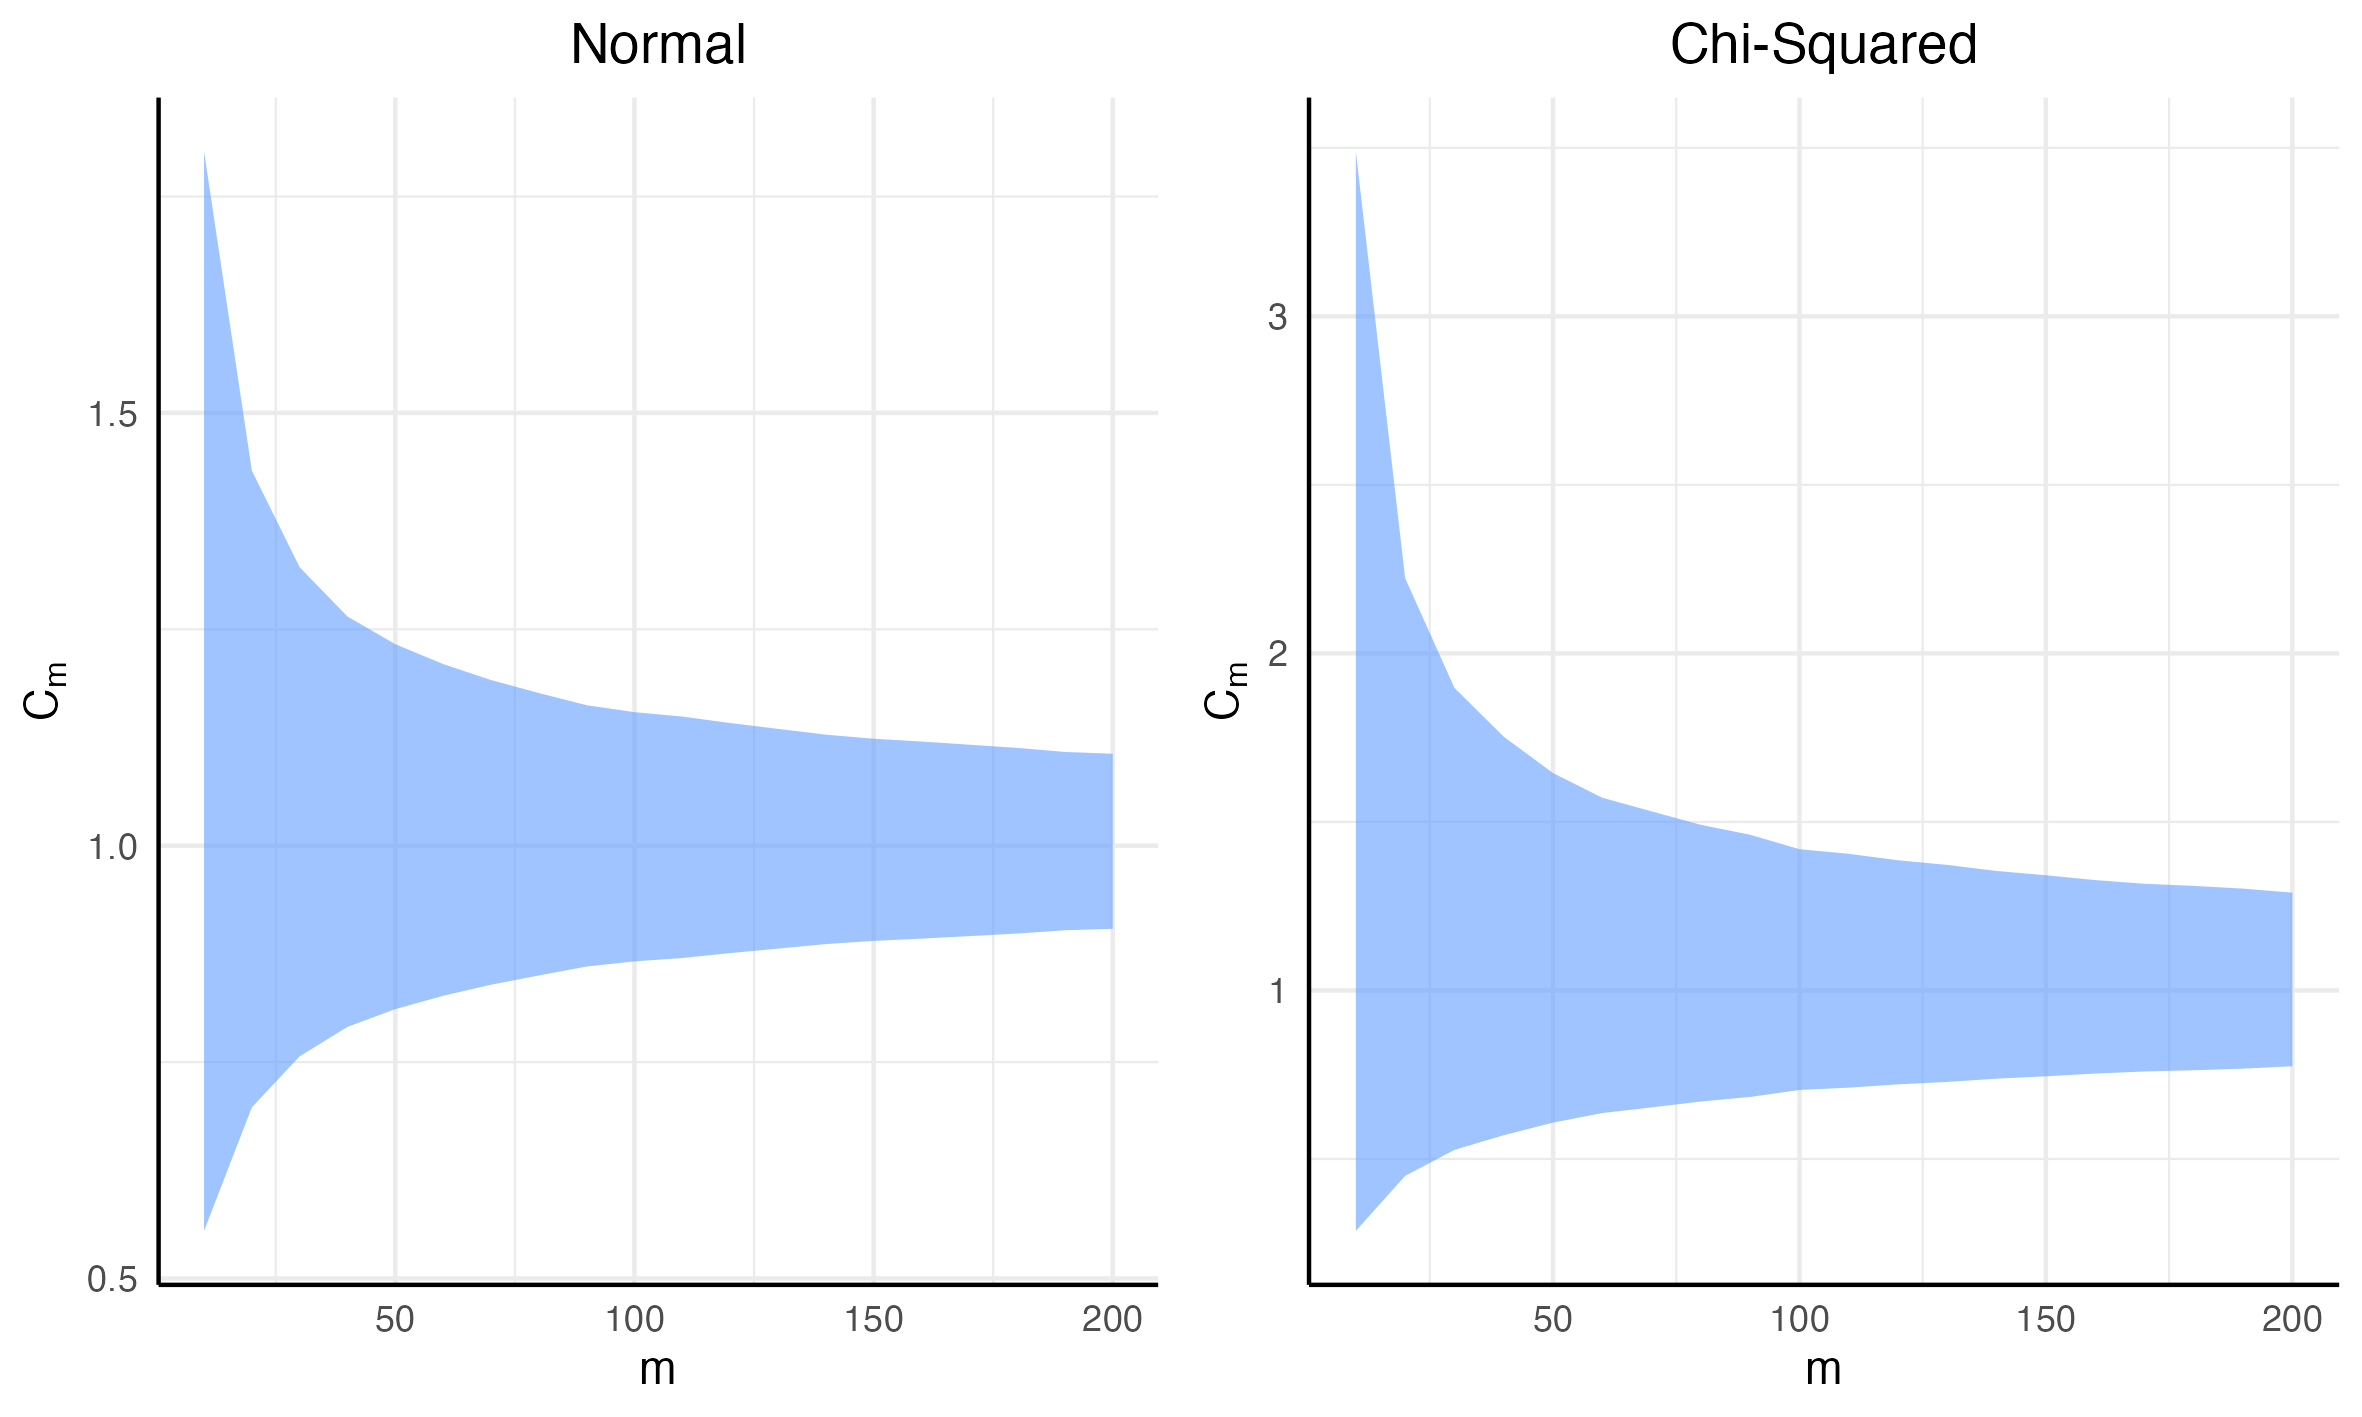
\includegraphics[width=\linewidth]{normchisq}
  \column{.25\linewidth}
  \begin{itemize}
    \item \textbf{Left:} Normal. \(C_{20} = [0.70, 1.43]\),
      \(C_{50} = [0.81, 1.23]\).
    \vfill
    \item \textbf{Right:} \(\chi^{2}_{1}\). \(C_{20} = [0.49, 2.22]\),
      \(C_{50} = [0.64, 1.61]\).
  \end{itemize}
\end{columns}
\vfill
Higher kurtosis \(\Rightarrow\) wider \(C_m\).
\end{frame}

\begin{frame}
\frametitle{How wide is \(C_{m}\): Pareto DGPs}
\centering
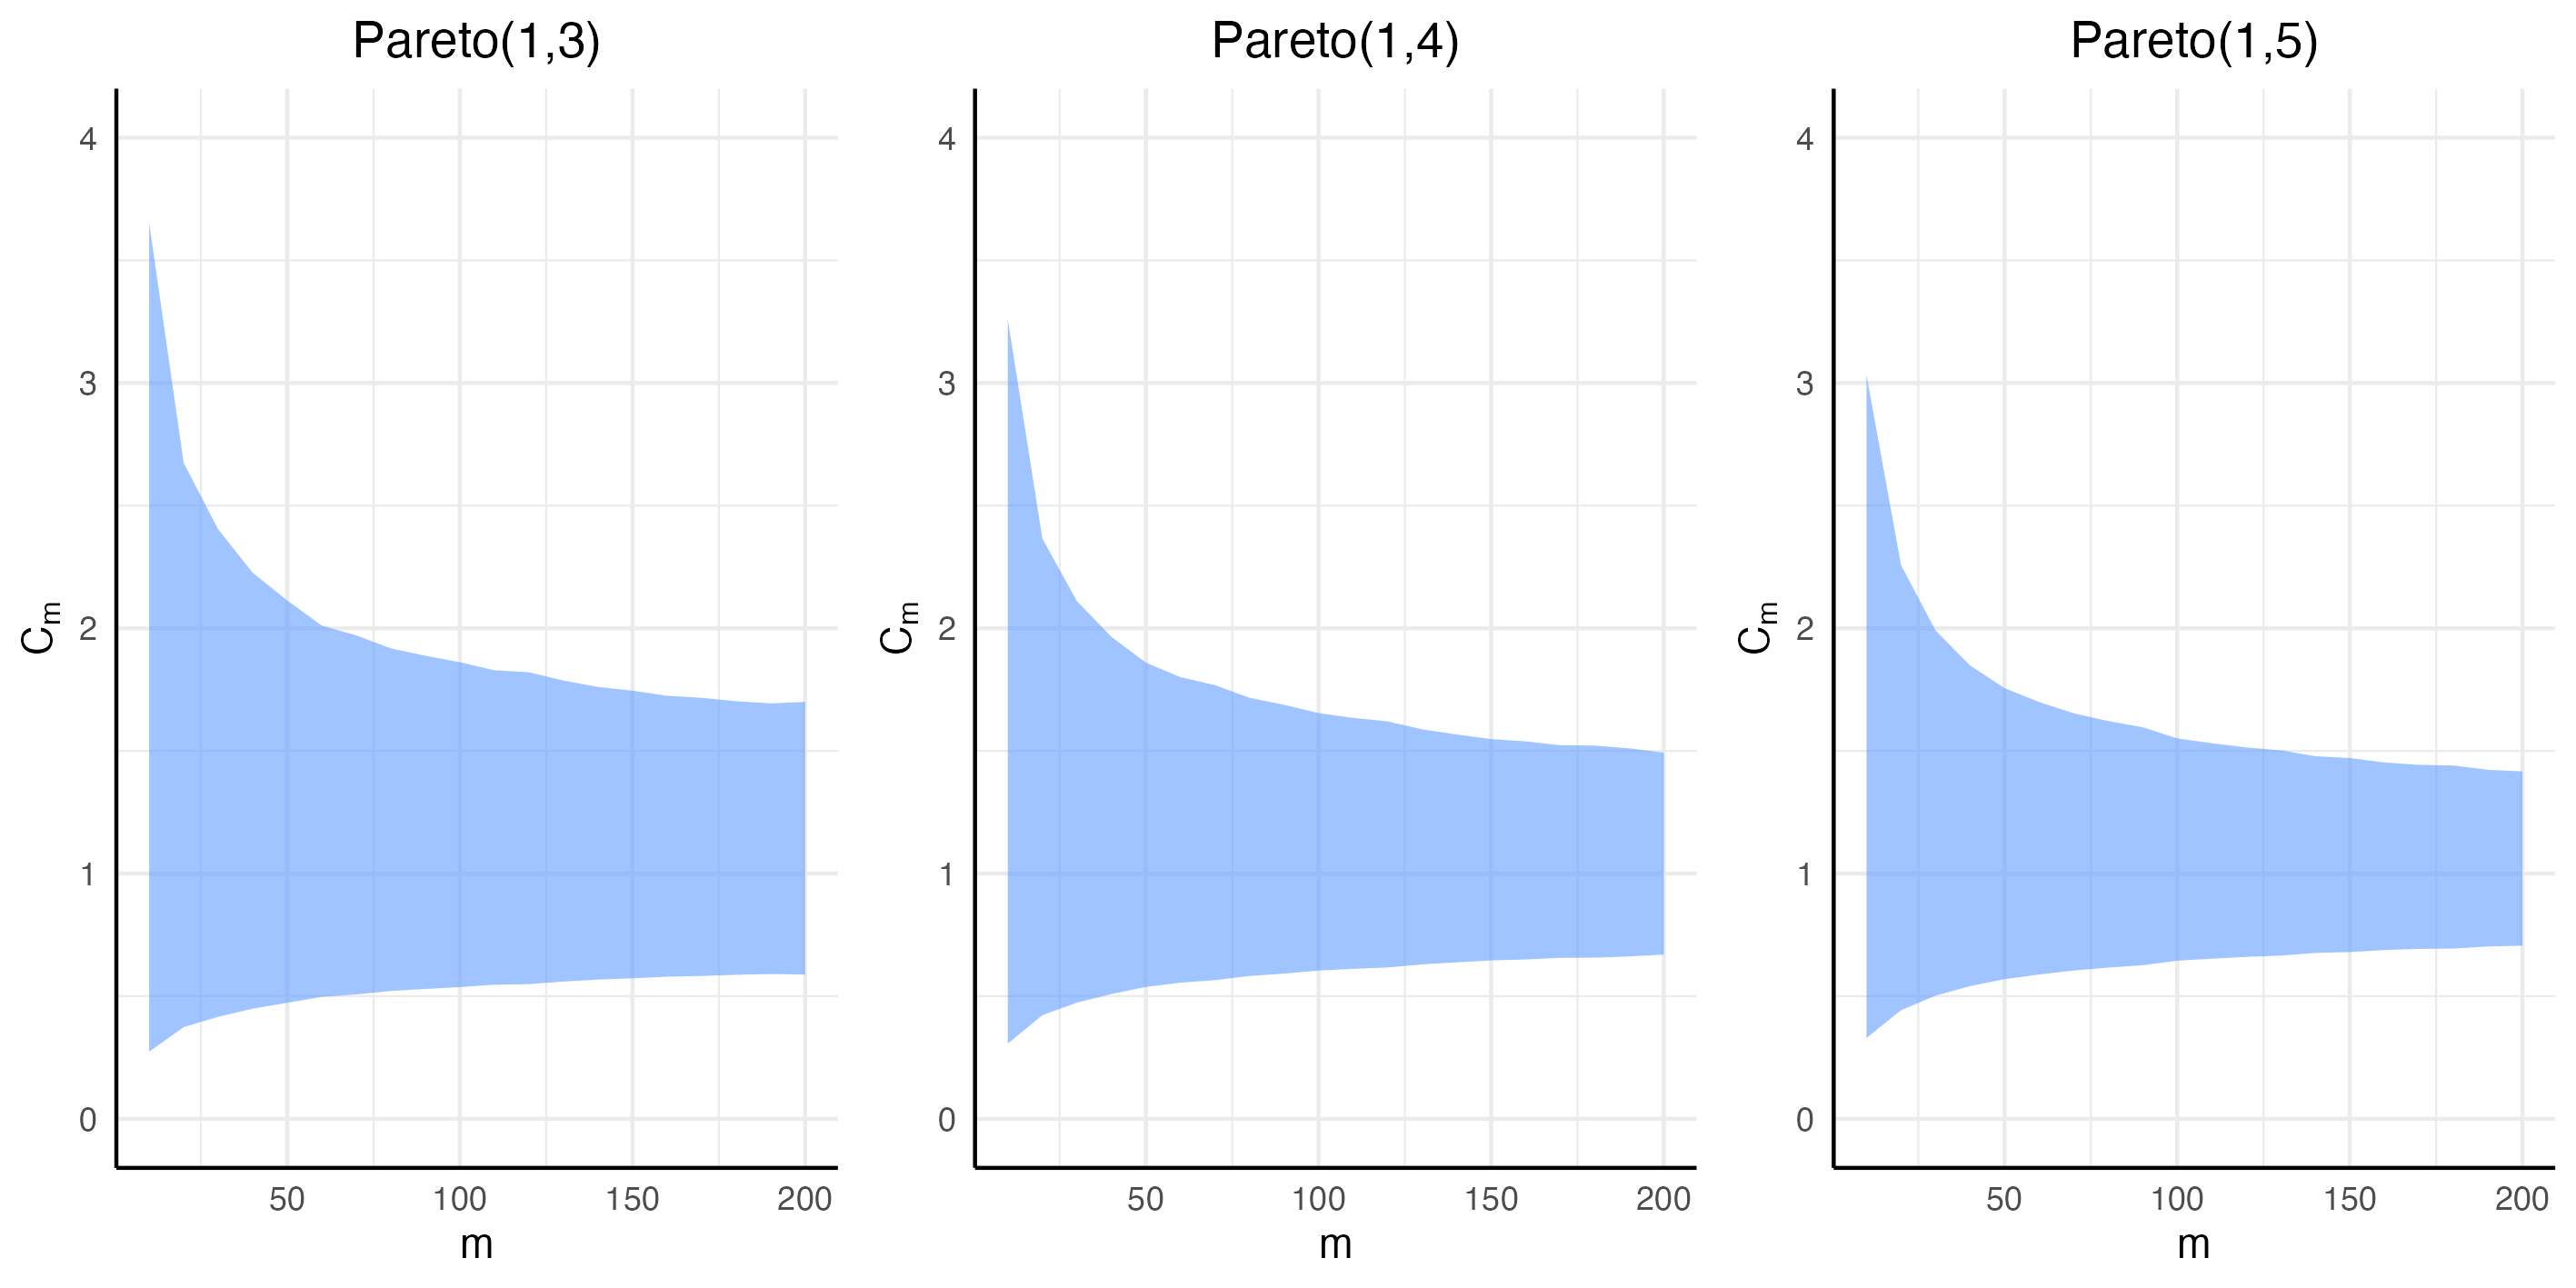
\includegraphics[width=.9\linewidth]{pareto}
\vfill
\(Y(a) \sim \mu(a) + \sigma(a)\cdot \text{Pareto}(1, s)\),
\(s \in \{3,4,5\}\) (left to right).
\vfill
For \(s = 3\), \(C_{50} = [0.50, 2.15]\) -- a substantial range.
\end{frame}

\begin{frame}
\frametitle{Approximating \(C_{m}\) under sub-Gaussianity}
\begin{prop*}
If \(Y (a)\) are sub-Gaussian,

then as \(m \to \infty\),
\begin{equation*}
  C_{m} = \left[ 1 - m^{-1/2} V + \delta_{m}^{-},
  1 + m^{-1/2} V + \delta_{m}^{+} \right]
\end{equation*}
where \(\delta_{m}^{-}, \delta_{m}^{+} = o (m^{-1/2})\) as \(m \to \infty\) and
\begin{equation*}
  V = \frac{1}{4} \left( \frac{\E [(Y (1) - \mu (1))^{4}]}{\sigma^{4} (1)}
  + \frac{\E [(Y(0) - \mu(0))^{4}]}{\sigma^{4} (0)} - 2 \right).
\end{equation*}
\end{prop*}
\vfill
\begin{itemize}
  \item \(|C_m|\) shrinks to zero at rate \(1/\sqrt m\), with constant
    \(V\) dependent on \textbf{kurtosis}.
    \vfill
  \item Even with bounded outcomes, FNA is sensitive to heavy tails.
\end{itemize}
\end{frame}

\begin{frame}
\frametitle{Efficiency loss: how bad can it get?}
\begin{defn*}[Efficiency loss of FNA vs.\ BA]
\begin{equation*}
  \mathcal{L}^{d} (F) =
  \E_{F} \left[ \frac{\sigma_{F}^{2} (1)}{\tilde{\pi}} + \frac{\sigma_{F}^{2}
  (0)}{1 - \tilde{\pi}} \right] - 2 (\sigma_{F}^{2} (1) + \sigma_{F}^{2} (0)),
  \qquad
  \mathcal{L}^{r} (F) = \frac{\E_{F} \left[ \frac{\sigma_{F}^{2}
  (1)}{\tilde{\pi}} + \frac{\sigma_{F}^{2} (0)}{1 - \tilde{\pi}}
  \right]}{2 (\sigma_{F}^{2} (1) + \sigma_{F}^{2} (0))}.
\end{equation*}
\end{defn*}
\vfill
\begin{prop*}
Under fixed-\(m\) asymptotics, with
\(\mathcal{F}(K) = \{F : 0 < \sigma_{F}^{2} (0), \sigma_{F}^{2} (1) \leq K\}\):
\begin{align*}
  \sup_{F \in \mathcal{F}(K)} \mathcal{L}^d (F) =
  & \, +\infty,
  & \inf_{F \in \mathcal{F}(K)} \mathcal{L}^d (F) =
  & \, -K, \\
  \sup_{F \in \mathcal{F}(K)}\!\mathcal{L}^r(F) =
  & \, \infty,
  & \inf_{F \in \mathcal{F}(K)}\!\mathcal{L}^r(F) =
  & \, \tfrac{1}{2}.
\end{align*}
\end{prop*}
\vfill
In terms of regret, BA dominates FNA.
\end{frame}

\begin{frame}
\frametitle{Efficiency loss: main ideas}
Can show
\begin{equation*}
  \calL^{d} = 2 \sigma (1) \sigma (0) (B_{m} - 1) - (\sigma (1) - \sigma
  (0))^{2} \qquad \text{and} \qquad
  \calL^{r} = \frac{1}{2} + B_{m} \frac{\sigma (1) \sigma (0)}{\sigma^{2} (1) +
  \sigma^{2} (0)}.
\end{equation*}
\vfill
\pause

For fixed \(B_{m} > 1\):
\vfill
\begin{itemize}
  \item Lower bounds over \(\calF (K)\): fix \(\sigma^{2} (0) = K\) and push
    \(\sigma^{2} (1) \downarrow 0\)
    \begin{itemize}
      \item \(\calL^{d} \downarrow -K\); \(\calL^{r} = \frac{1}{2} + B_{m}
        \frac{\sigma (1) K^{1/2}}{\sigma^{2} (1) + K} \downarrow \frac{1}{2}\)
    \end{itemize}
    \vfill
  \item Upper bounds over \(\calF (K)\): for \(\sigma^{2} (a) = K\),
    \begin{itemize}
      \item \(\calL^{d} = 2 K (B_{m} - 1)\); \(\calL^{r} = (1 + B_{m}) / 2\).
    \end{itemize}
\end{itemize}
\vfill
\pause

Key idea for upper bounds:
\vfill
\begin{itemize}
  \item \(B_{m}\) is an expectation of ratios of unit variance random variables.
    \vfill
  \item Unit variance does not control magnitude of expectations of ratios:
    there exist sequences of DGPs \(\{F_{j}\} \subseteq \calF (K)\) such that
    \(B_{m} (F_{j}) \to \infty\) as \(j \to \infty\) with both \(m\) and \(K\)
    fixed!
\end{itemize}
\end{frame}

%%%%%%%%%%%%%%%%%%%%%%%%%%%%%%%%%%%%%%%%%%%%%%%%%%%%%%%%%%%%%%%%%%%%%%%%%%%%%%%%
\section{Simulation evidence}
%%%%%%%%%%%%%%%%%%%%%%%%%%%%%%%%%%%%%%%%%%%%%%%%%%%%%%%%%%%%%%%%%%%%%%%%%%%%%%%%

\begin{frame}[plain,noframenumbering]
  \frametitle{Outline}
  \tableofcontents[currentsection]
\end{frame}

\begin{frame}
\frametitle{Simulation setup}
\(Y(1) = 0.075 + \sigma(1)\varepsilon(1),\quad
  Y(0) = \sigma(0)\varepsilon(0),\quad
  \sigma^2(1) + \sigma^2(0) = 2\).
\vfill
Five DGPs for errors (each standardized to mean 0 var 1):
\vfill
\begin{itemize}
  \item \textbf{Model 1:} \(\Normal(0,1)\) -- thin tails.
    \vfill
  \item \textbf{Model 2:} standardized \(\chi^2_1\) -- moderate tails.
    \vfill
  \item \textbf{Model 3-5:} standardized \(\text{Pareto}(1,s)\),
    \(s \in \{3,4,5\}\) -- heavy tails.
\end{itemize}
\vfill
Pilot: \(m = 20\); main wave: \(n = 1000\); \(10^{5}\) Monte Carlo draws per
\(\sigma(1)/\sigma(0) \in (0,1]\).
\vfill
Plot MSE of FNA vs.\ BA vs.\ INA as functions of \(\sigma(1)/\sigma(0)\).
\end{frame}

\begin{frame}
\frametitle{MSE: Normal and \(\chi^2_1\), \(m = 20\)}
\centering
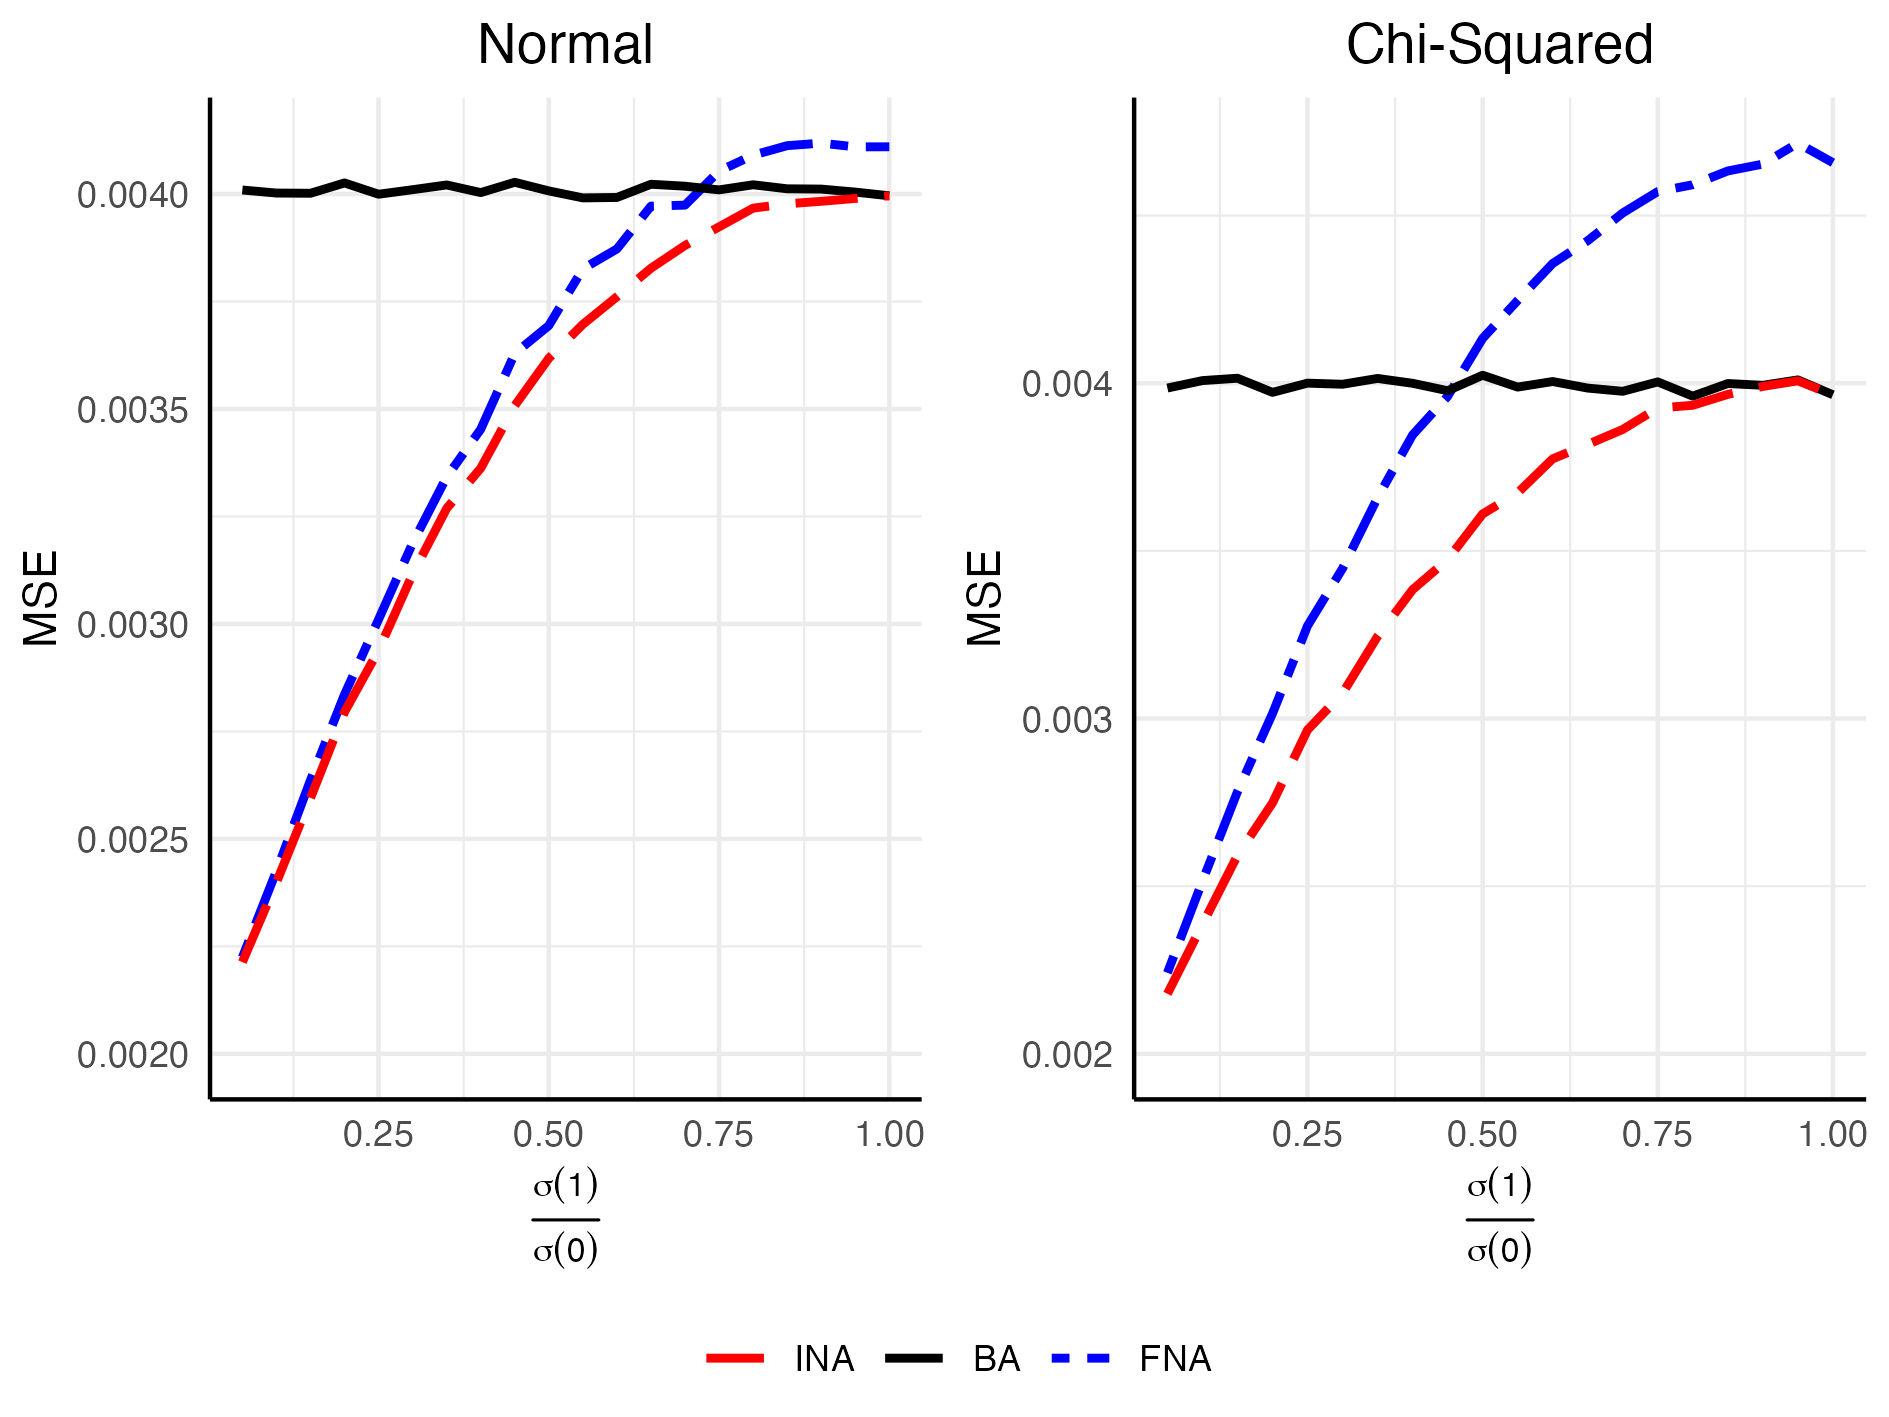
\includegraphics[width=.6\linewidth]{MSE_12}
\vfill
\begin{itemize}
  \item \textbf{Normal:} FNA is \(\approx 3\%\) worse than BA at
    homoskedasticity.
    \vfill
  \item \textbf{\(\chi^2_1\):} FNA is \(\approx 17\%\) worse for
    \(\sigma(1)/\sigma(0) \in [0.75, 1]\).
\end{itemize}
\end{frame}

\begin{frame}[allowframebreaks]
\frametitle{MSE: Pareto, \(m = 20\)}
\centering
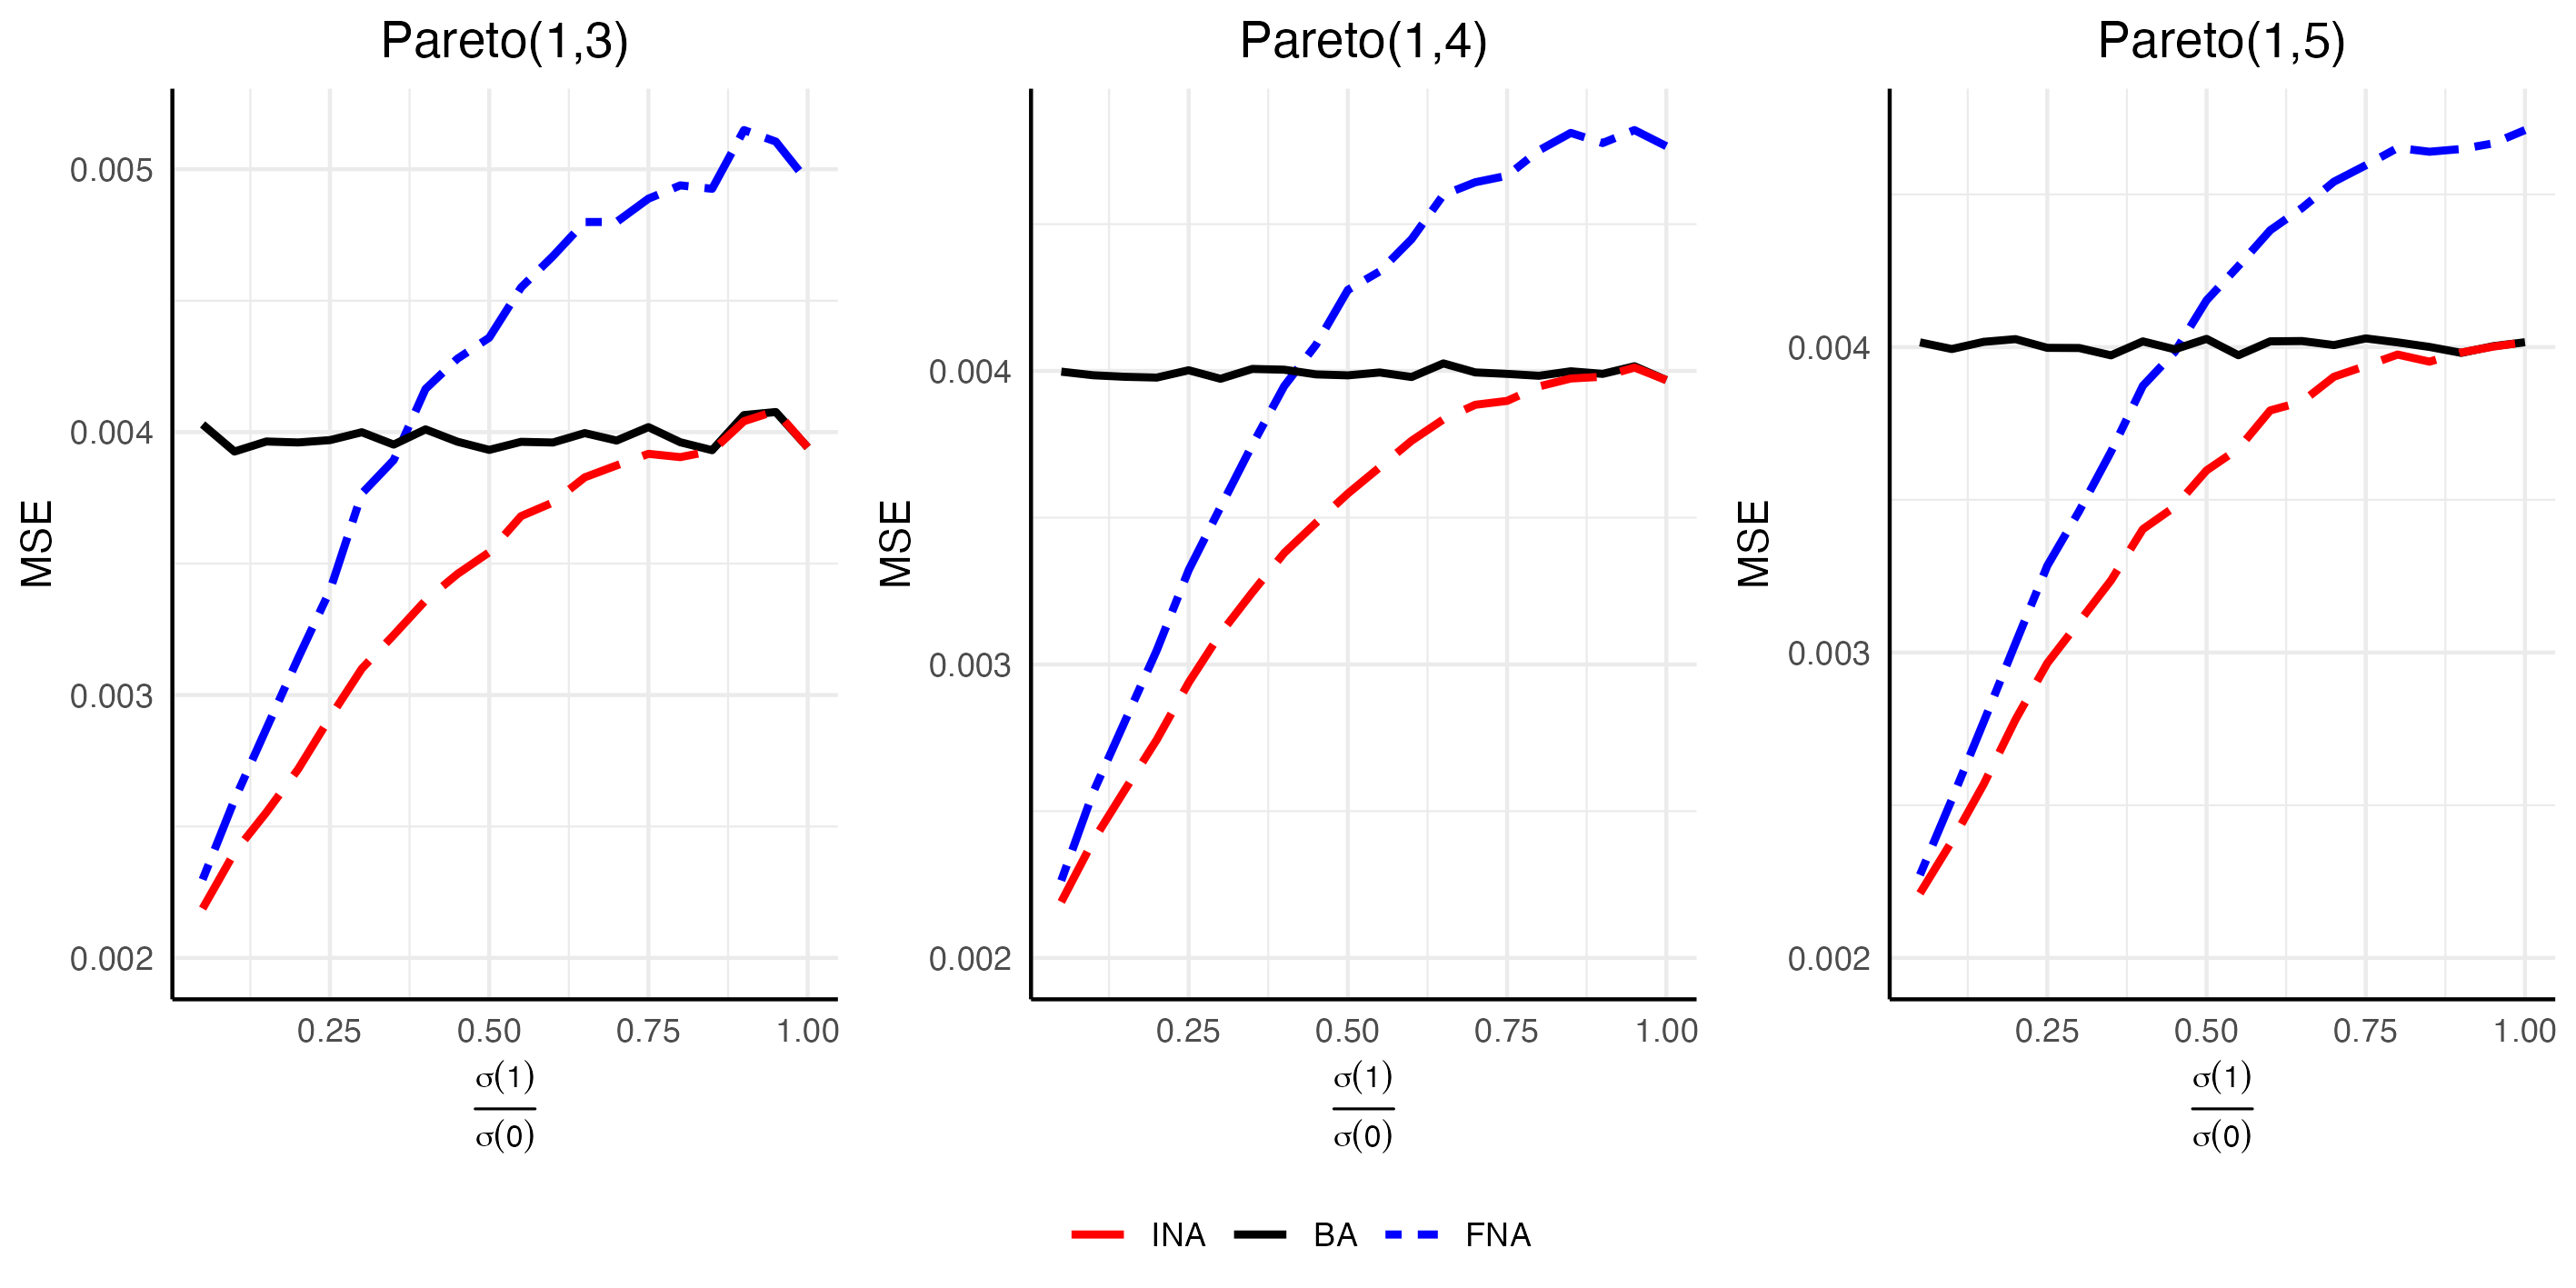
\includegraphics[width=0.9\linewidth]{MSE_345}
\vfill

For \(s = 3,4,5\) (left to right), at homoskedasticity FNA is \(26\%\),
\(20\%\), \(17\%\) worse than BA.
\vfill

At \(m = 50\), losses shrink to roughly \(13\%\), \(11\%\), \(8.6\%\) -- but
remain non-trivial.
\end{frame}

%%%%%%%%%%%%%%%%%%%%%%%%%%%%%%%%%%%%%%%%%%%%%%%%%%%%%%%%%%%%%%%%%%%%%%%%%%%%%%%%
\section{How common is the problem? Evidence from RCTs}
%%%%%%%%%%%%%%%%%%%%%%%%%%%%%%%%%%%%%%%%%%%%%%%%%%%%%%%%%%%%%%%%%%%%%%%%%%%%%%%%

\begin{frame}[plain,noframenumbering]
  \frametitle{Outline}
  \tableofcontents[currentsection]
\end{frame}

\begin{frame}
\frametitle{Empirical strategy}
\begin{itemize}
  \item Look at first 10 completed experiments with pub. avail. data
    in AER RCT Registry.
    \vfill
  \item For each experiment, ask:
    \emph{If these authors had run a small pilot from the same population,
    would they have done better with FNA or with BA?}
    \vfill
  \item Use the full experiment to estimate \(\sigma(0), \sigma(1)\) and check
    whether the ratio is close to 1.
    \vfill
  \item Two illustrative cases here:
    \vfill
    \begin{itemize}
      \item \citet{2014avvisatiGettingParentsInvolved}: relatively
        homoskedastic.
        \vfill
      \item \citet{2006ashrafTyingOdysseusMast}: heteroskedastic but
        heavy-tailed.
    \end{itemize}
\end{itemize}
\end{frame}

\begin{frame}
\frametitle{\citet{2014avvisatiGettingParentsInvolved}: Parental Involvement in French Schools}
\centering\small
\begin{tabular}{lccc}
\toprule
Outcome (student-level) & Treat. & Cont. & Treat./Cont. \\
\midrule
Global parenting score              & 0.34 & 0.34 & 1.01 \\
School-based involvement            & 0.66 & 0.63 & 1.05 \\
Pedagogical team: behavior          & 0.73 & 0.74 & 0.98 \\
Pedagogical team: discipline        & 1.20 & 1.18 & 1.02 \\
French (uniform test)               & 0.99 & 1.01 & 0.98 \\
Mathematics (uniform test)          & 0.99 & 1.02 & 0.98 \\
\bottomrule
\end{tabular}
\vfill
\begin{itemize}
  \item Ratios extremely close to 1 across most outcomes.
    \vfill
  \item For \(m = 20\) normal pilot, \(C_{20} = [0.70, 1.43]\) -- nearly all
    outcomes fall inside.
    \vfill
  \item \textbf{BA would beat FNA in this design.}
\end{itemize}
\end{frame}

\begin{frame}
\frametitle{\citet{2006ashrafTyingOdysseusMast}: Commitment Savings in the Philippines}
Treatment effect on \textbf{change in total balance} over 6 and 12 months:
\vfill
\centering\small
\begin{tabular}{lccccc}
\toprule
Outcome                                & Treat.\ SD & Marketing \ SD &  Cont.\ SD & T/M & T/C \\
\midrule
\(\Delta\) Tot.\ Bal.\ (6m)            & 2347.6 & 2880.7 & 1336.0 & 0.81 & 1.76 \\
\(\Delta\) Tot.\ Bal.\ (12m)           & 6093.2 & 1945.0 & 2690.7 & 3.13 & 2.26 \\
\(\Delta\) Tot.\ Bal.\ \(>0\%\) (12m)  & 0.47   & 0.45   & 0.42   & 1.05 & 1.11 \\
\(\Delta\) Tot.\ Bal.\ \(>20\%\) (12m) & 0.40   & 0.35   & 0.31   & 1.16 & 1.30 \\
\bottomrule
\end{tabular}
\vfill
\flushleft
\begin{itemize}
  \item Continuous outcomes look heteroskedastic. (T/M = 3.13!)
    \vfill
  \item But also \emph{very} heavy-tailed: kurtosis ranges from 67 to a little
    over 300.
    \vfill
  \item So \(C_m\) is very wide. We can estimate it directly using the data -
    letting \(m\) range up to 2000.
\end{itemize}
\end{frame}

\begin{frame}
\frametitle{\(C_{m}\) in \citet{2006ashrafTyingOdysseusMast} --- 6 month
outcomes}
\centering
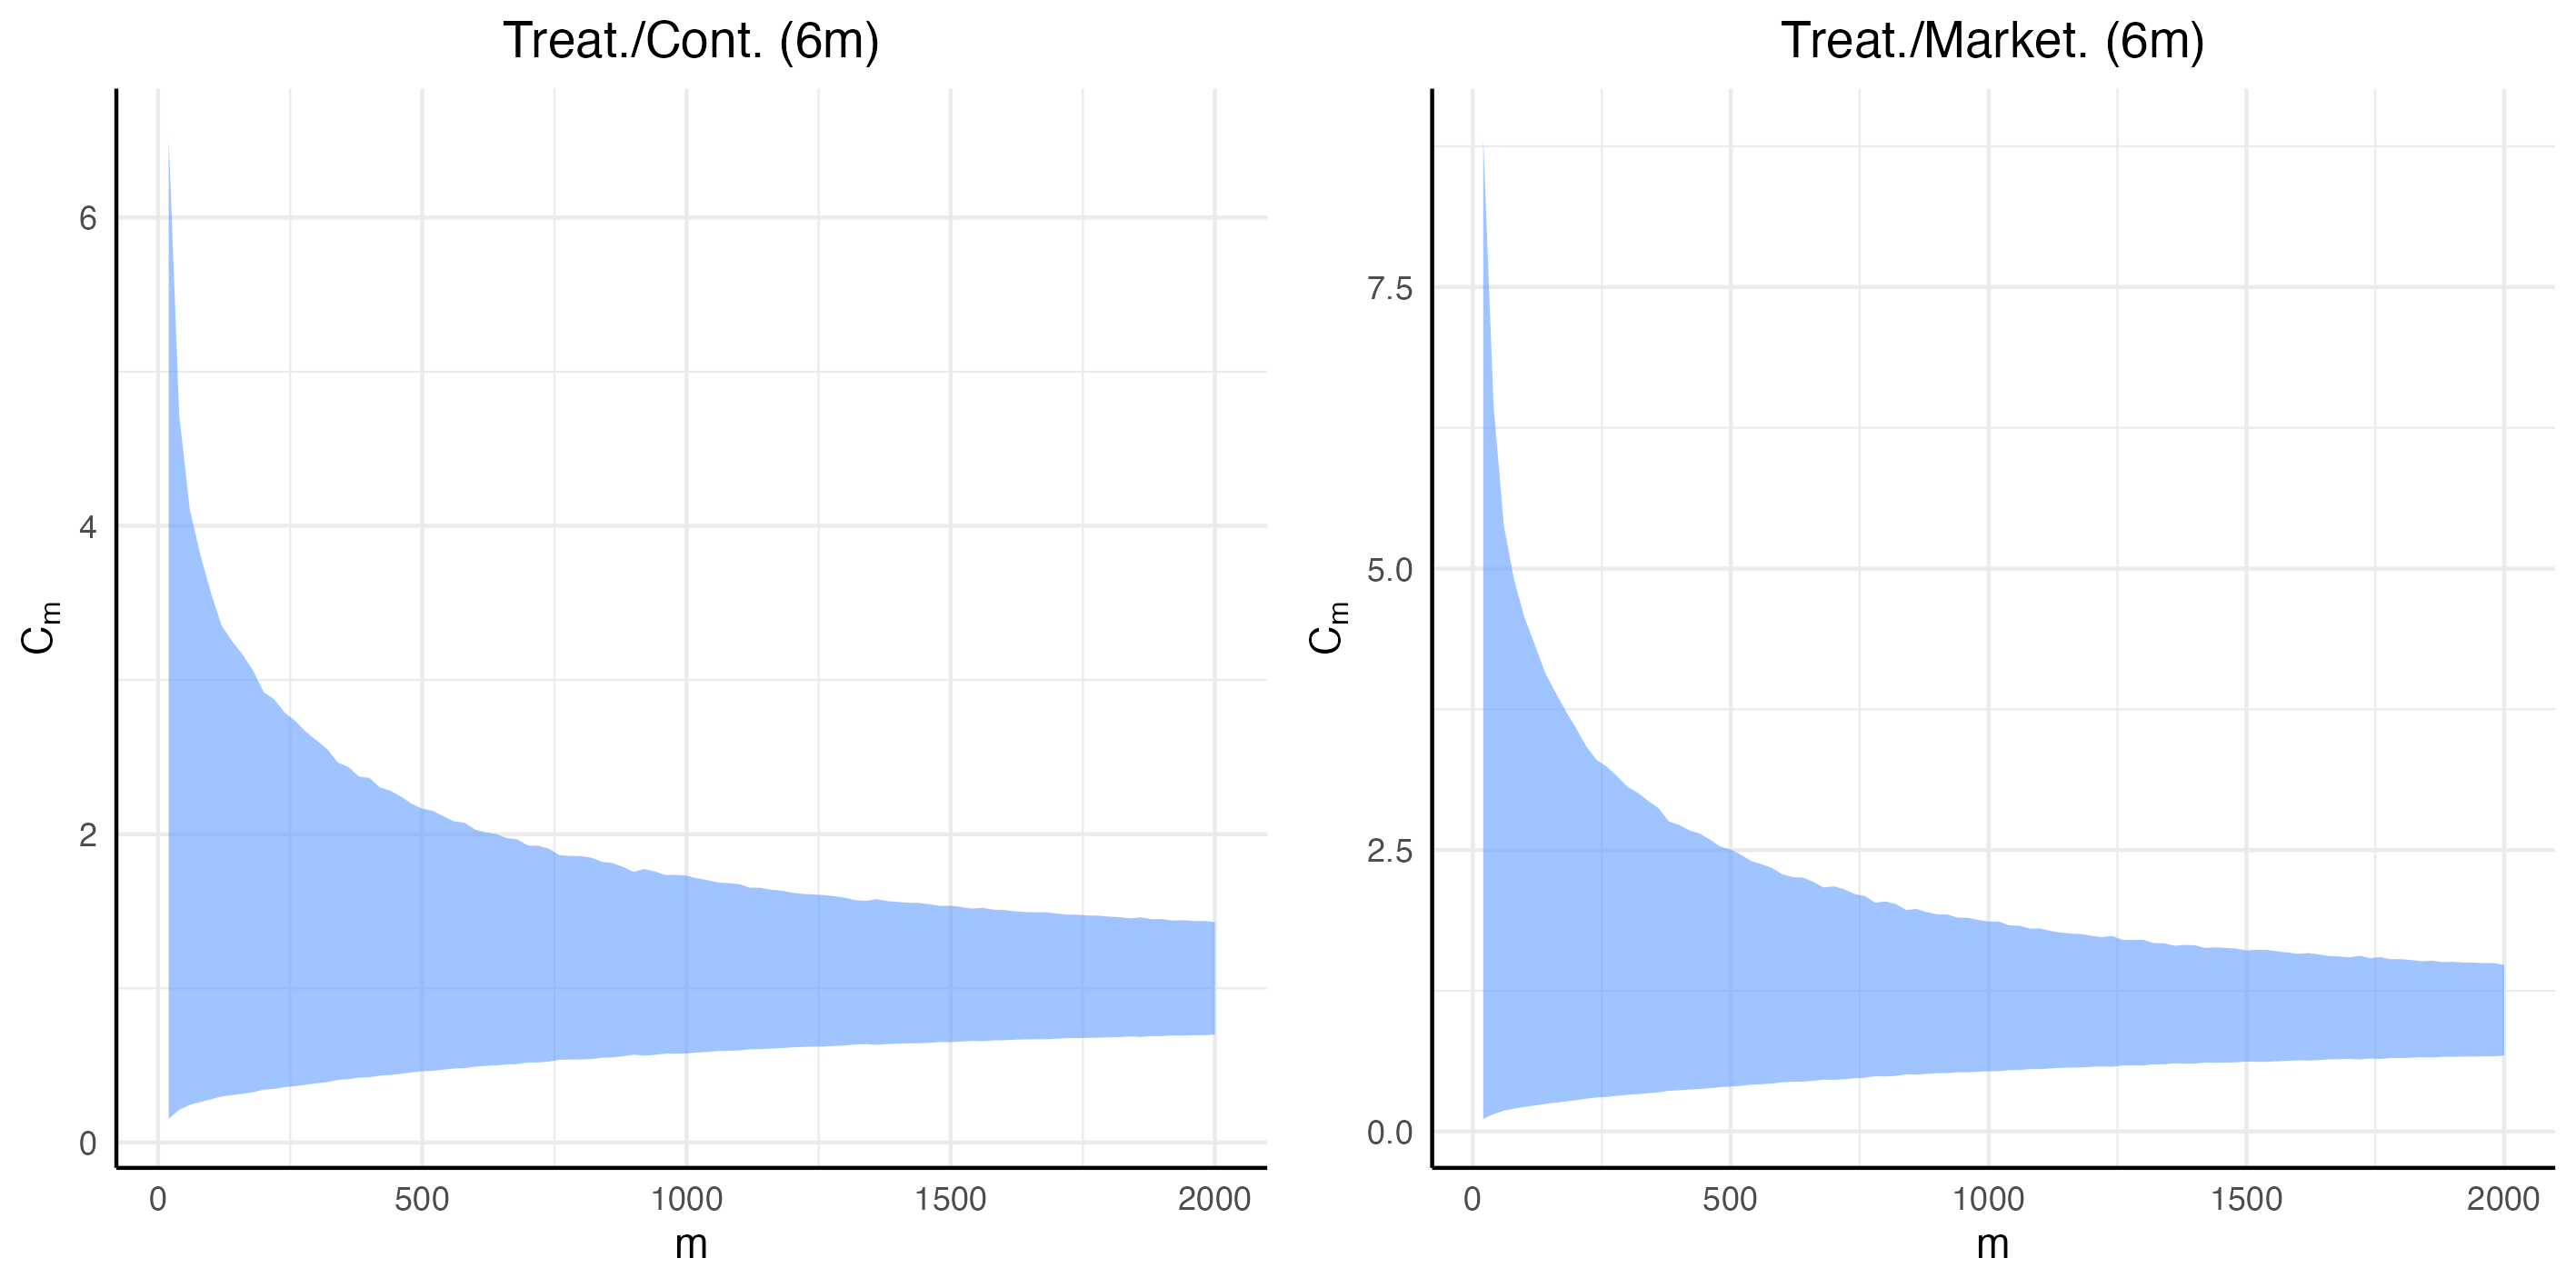
\includegraphics[scale=0.14]{balchange_combined_plot_1.png}
\end{frame}

\begin{frame}
\frametitle{\(C_{m}\) in \citet{2006ashrafTyingOdysseusMast} --- 12 month
outcomes}
\centering
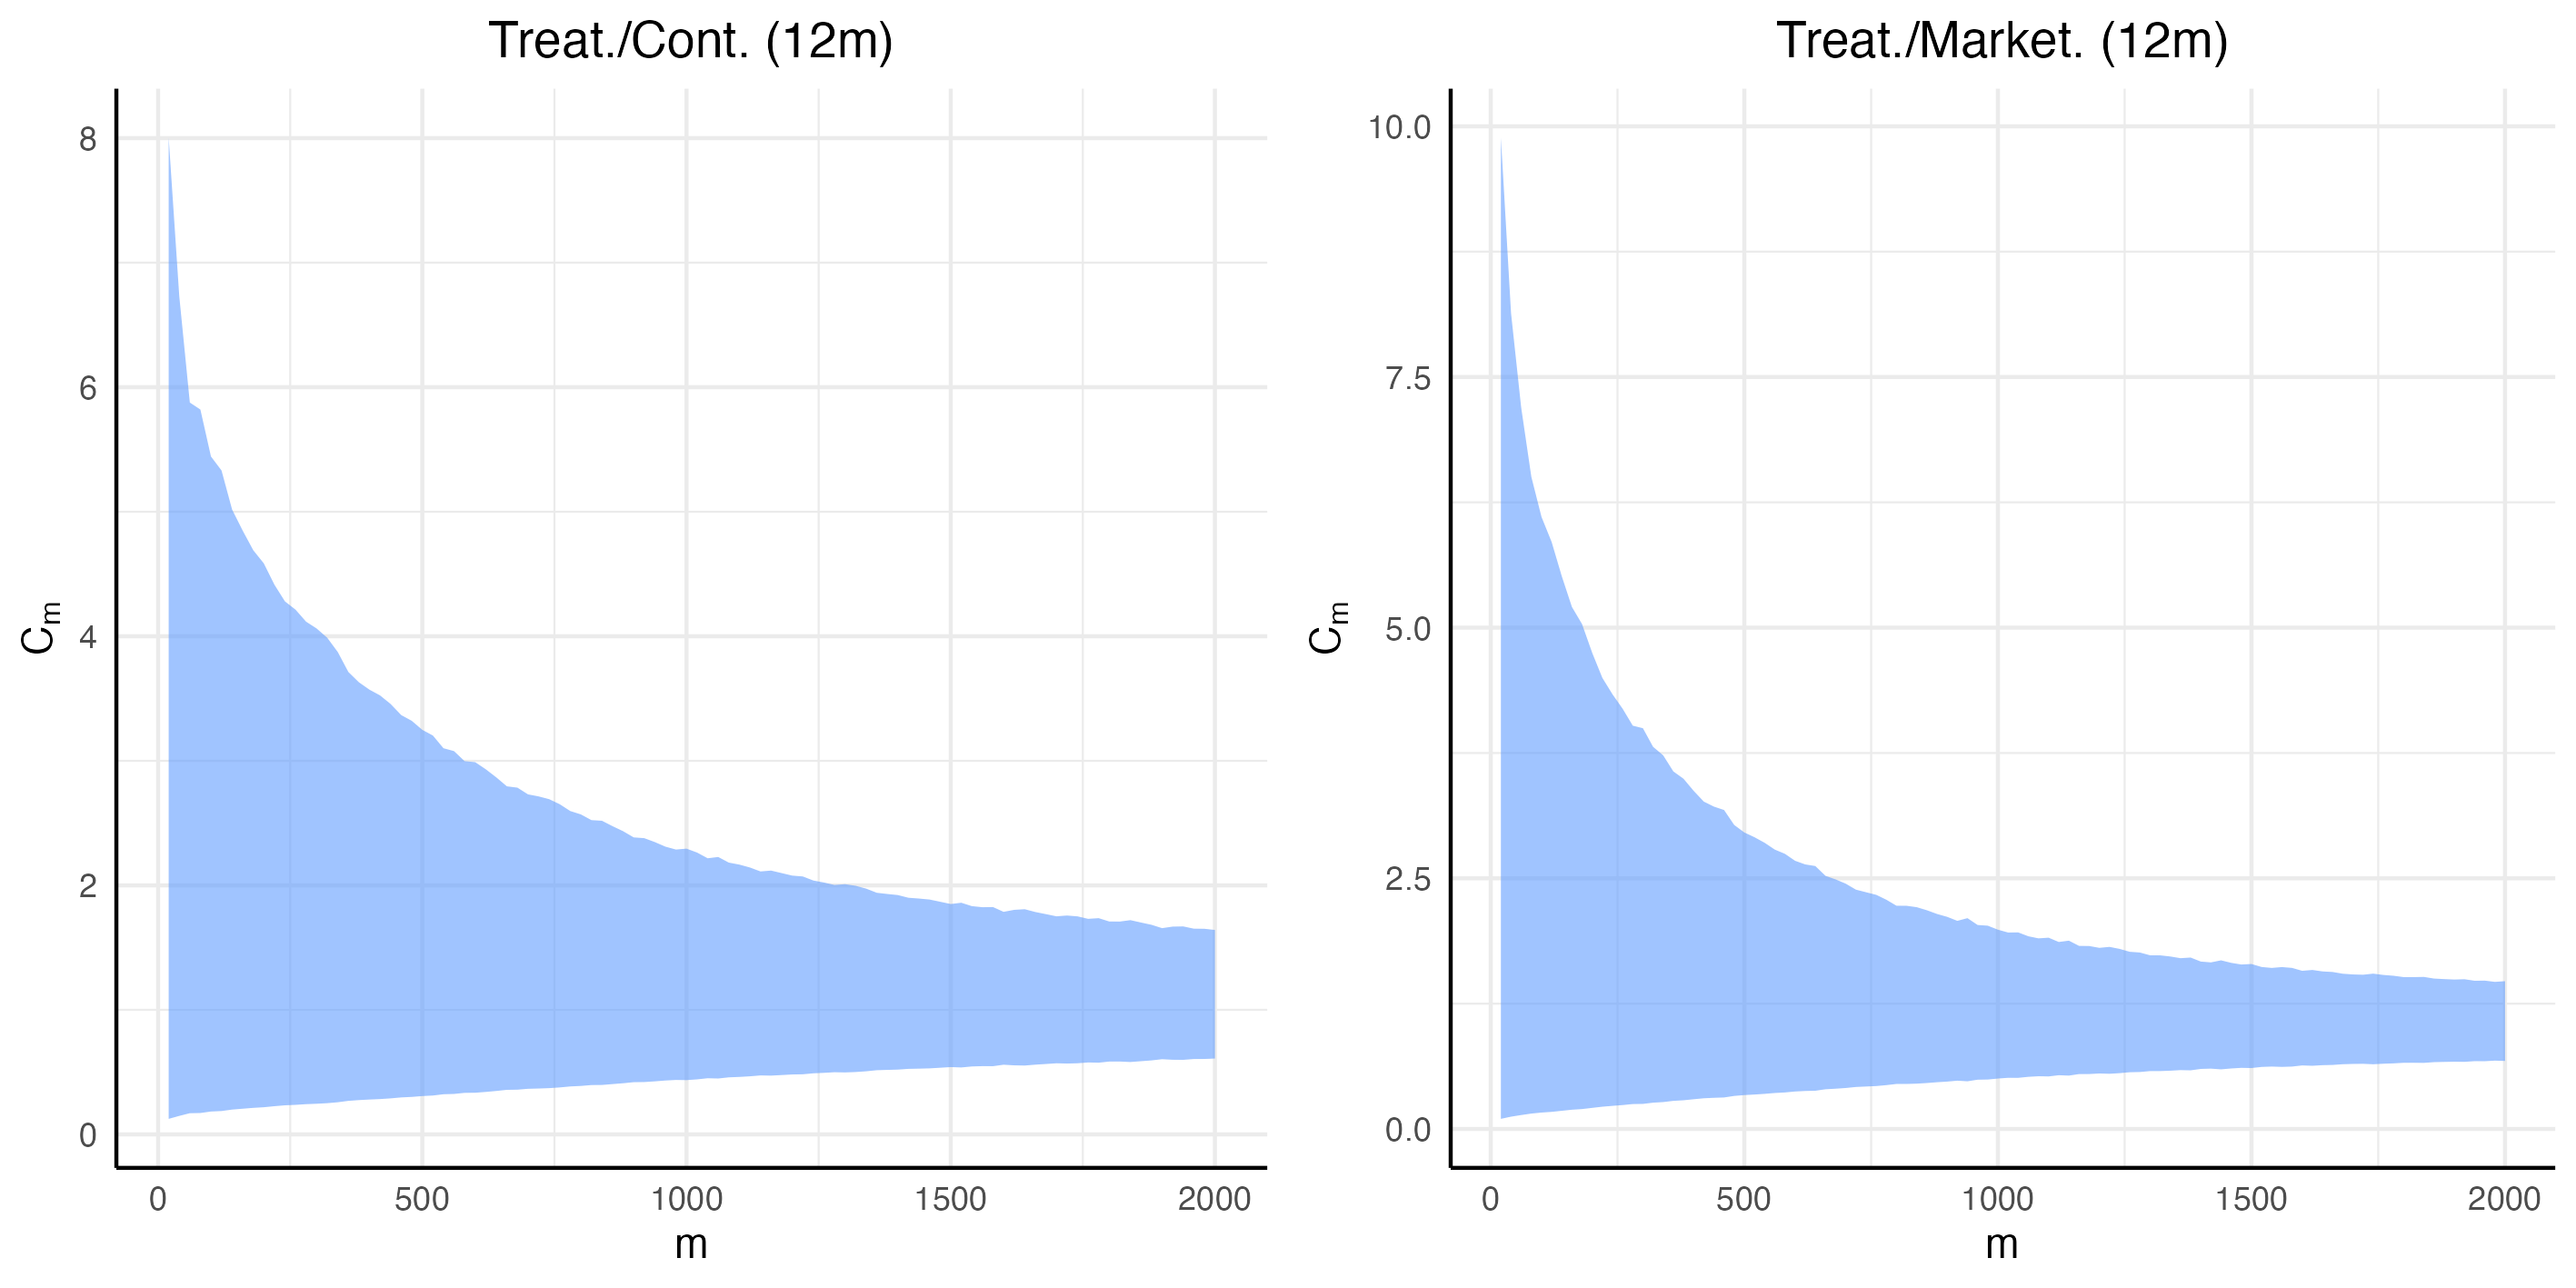
\includegraphics[scale=0.14]{balchange_combined_plot_2.png}
\end{frame}

\begin{frame}
\frametitle{Necessary pilot sizes for FNA to beat BA}
\centering\small
\begin{tabular}{lcc}
\toprule
Necessary pilot size       & T vs.\ M & T vs.\ C \\
\midrule
Exact 6m                   & --       & 931  \\
Exact 12m                  & 475      & 1015 \\
\midrule
Sub-Gaussian approx., 6m   & 6858     & 355  \\
Sub-Gaussian approx., 12m  & 36       & 177  \\
\bottomrule
\end{tabular}
\vfill
\begin{itemize}
  \item For T vs. M, the necessary pilot is over half the size of the actual
    experiment (\(n\) = 1777).
    \vfill
  \item For T vs. C at 6 months, sub-Gaussian approx. gives \(\sim 7000\) ---
    nearly 4\(\times\) experiment size.
    \vfill
  \item Sub-Gaussian asymptotics seem too optimistic for these data --- probably
    closer to Pareto.
    \vfill
  \item What about the remaining 8 experiments?
    \begin{itemize}
      \item BA beats FNA in 7/8 experiments due to relative homoskedasticity;
        \vfill
      \item Remaining experiment (\citet{2017mckenzieIdentifyingSpurringHigh})
        exhibits relative heteroskedasticity but outcomes have high kurtosis.
    \end{itemize}
\end{itemize}
\end{frame}

% %%%%%%%%%%%%%%%%%%%%%%%%%%%%%%%%%%%%%%%%%%%%%%%%%%%%%%%%%%%%%%%%%%%%%%%%%%%%%%
% \section{TODO: Potential Solutions}
% %%%%%%%%%%%%%%%%%%%%%%%%%%%%%%%%%%%%%%%%%%%%%%%%%%%%%%%%%%%%%%%%%%%%%%%%%%%%%%
%
% \begin{frame}[plain,noframenumbering]
%   \frametitle{Outline}
%   \tableofcontents[currentsection]
% \end{frame}
%
% \begin{frame}
% \frametitle{Three Candidate Solutions}
% The FNA fails because \(\tilde p\) is noisy. Pull it back toward
% \(1/2\)?
% \vfill
% \begin{enumerate}
%   \item \textbf{Pre-test for homoskedasticity:} Wald test on
%     \(\tilde\sigma^2(1) - \tilde\sigma^2(0) = 0\). Use FNA only
%     if rejected.
%     \vfill
%   \item \textbf{Additive regularization:}
%     \[
%       \tilde p^{\,\mathrm{add}}
%       = \frac{\tilde\sigma(1) + \nu\,\tilde\sigma(0)}
%              {(\tilde\sigma(1) + \tilde\sigma(0))(1+\nu)},
%       \quad \nu \ge 0.
%     \]
%     \vfill
%   \item \textbf{Exponential regularization:}
%     \[
%       \tilde p^{\,\mathrm{exp}}
%       = \frac{(\tilde\sigma(1)/\tilde\sigma(0))^{\tau}}
%              {1 + (\tilde\sigma(1)/\tilde\sigma(0))^{\tau}},
%       \quad \tau \in [0,1].
%     \]
%     \(\tau = 1\) recovers FNA; \(\tau = 0\) recovers BA.
% \end{enumerate}
% \end{frame}
%
% \begin{frame}
% \frametitle{Pre-Testing for Homoskedasticity}
% \centering
% 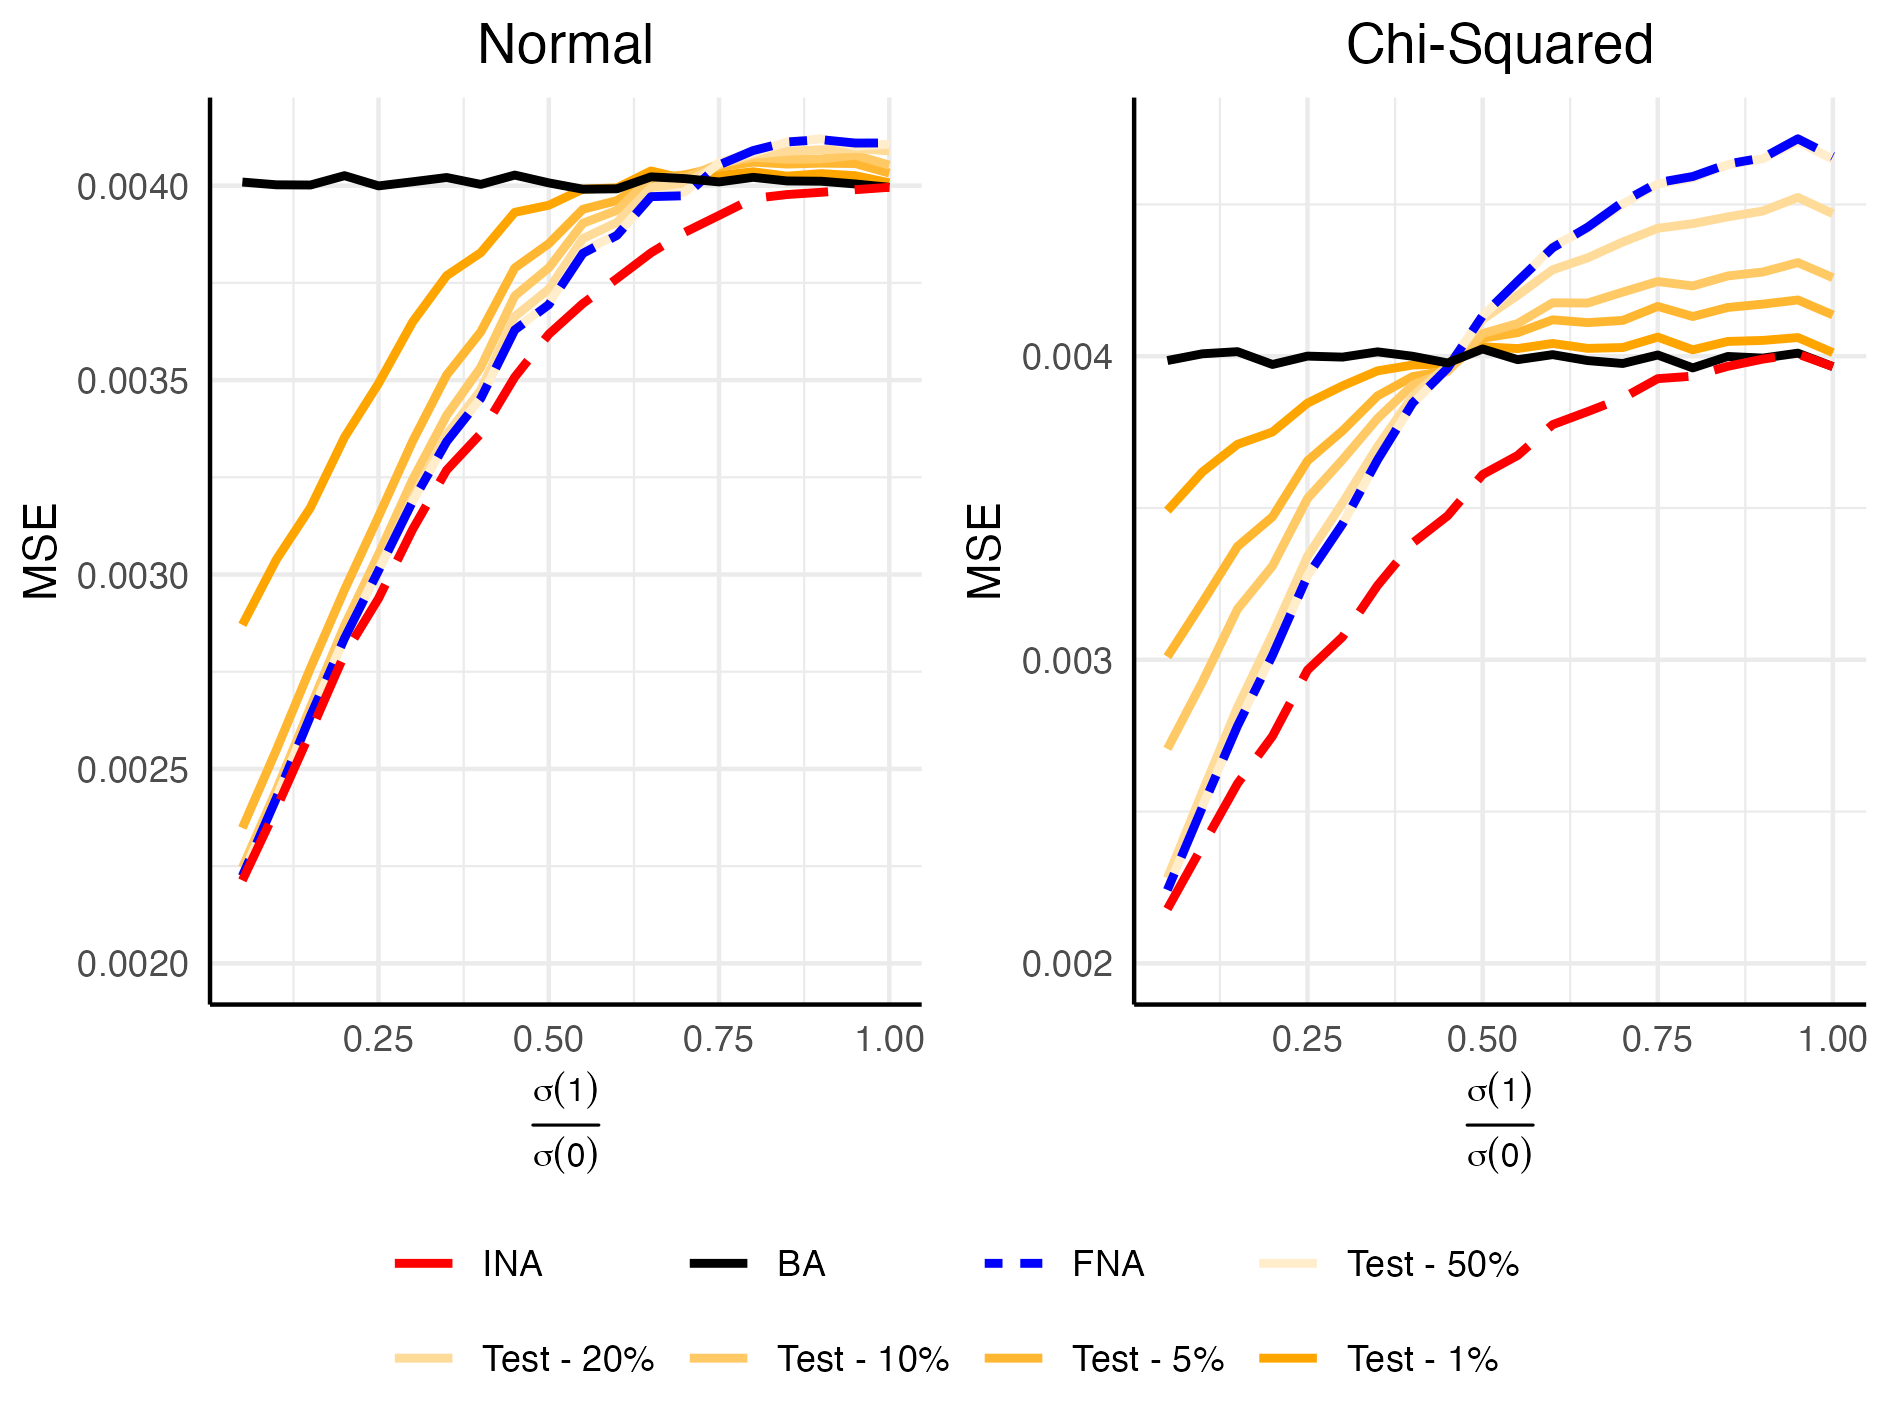
\includegraphics[width=.55\linewidth]{MSE_sol1_12}
% \vfill
% \begin{itemize}
%   \item \textcolor{red}{Red} = BA, \textcolor{blue}{blue} = FNA, oranges =
%     pre-test with \(\alpha \in \{1\%, 5\%, 10\%, 20\%, 50\%\}\).
%     \vfill
%   \item Smaller \(\alpha\) helps in homoskedastic region, hurts in
%     heteroskedastic region. Trade-off.
% \end{itemize}
% \end{frame}
%
% \begin{frame}
% \frametitle{Additive vs.\ Exponential Regularization}
% \begin{columns}
%   \column{.5\linewidth}
%   \centering
%   Additive (\(\nu\)) \\
%   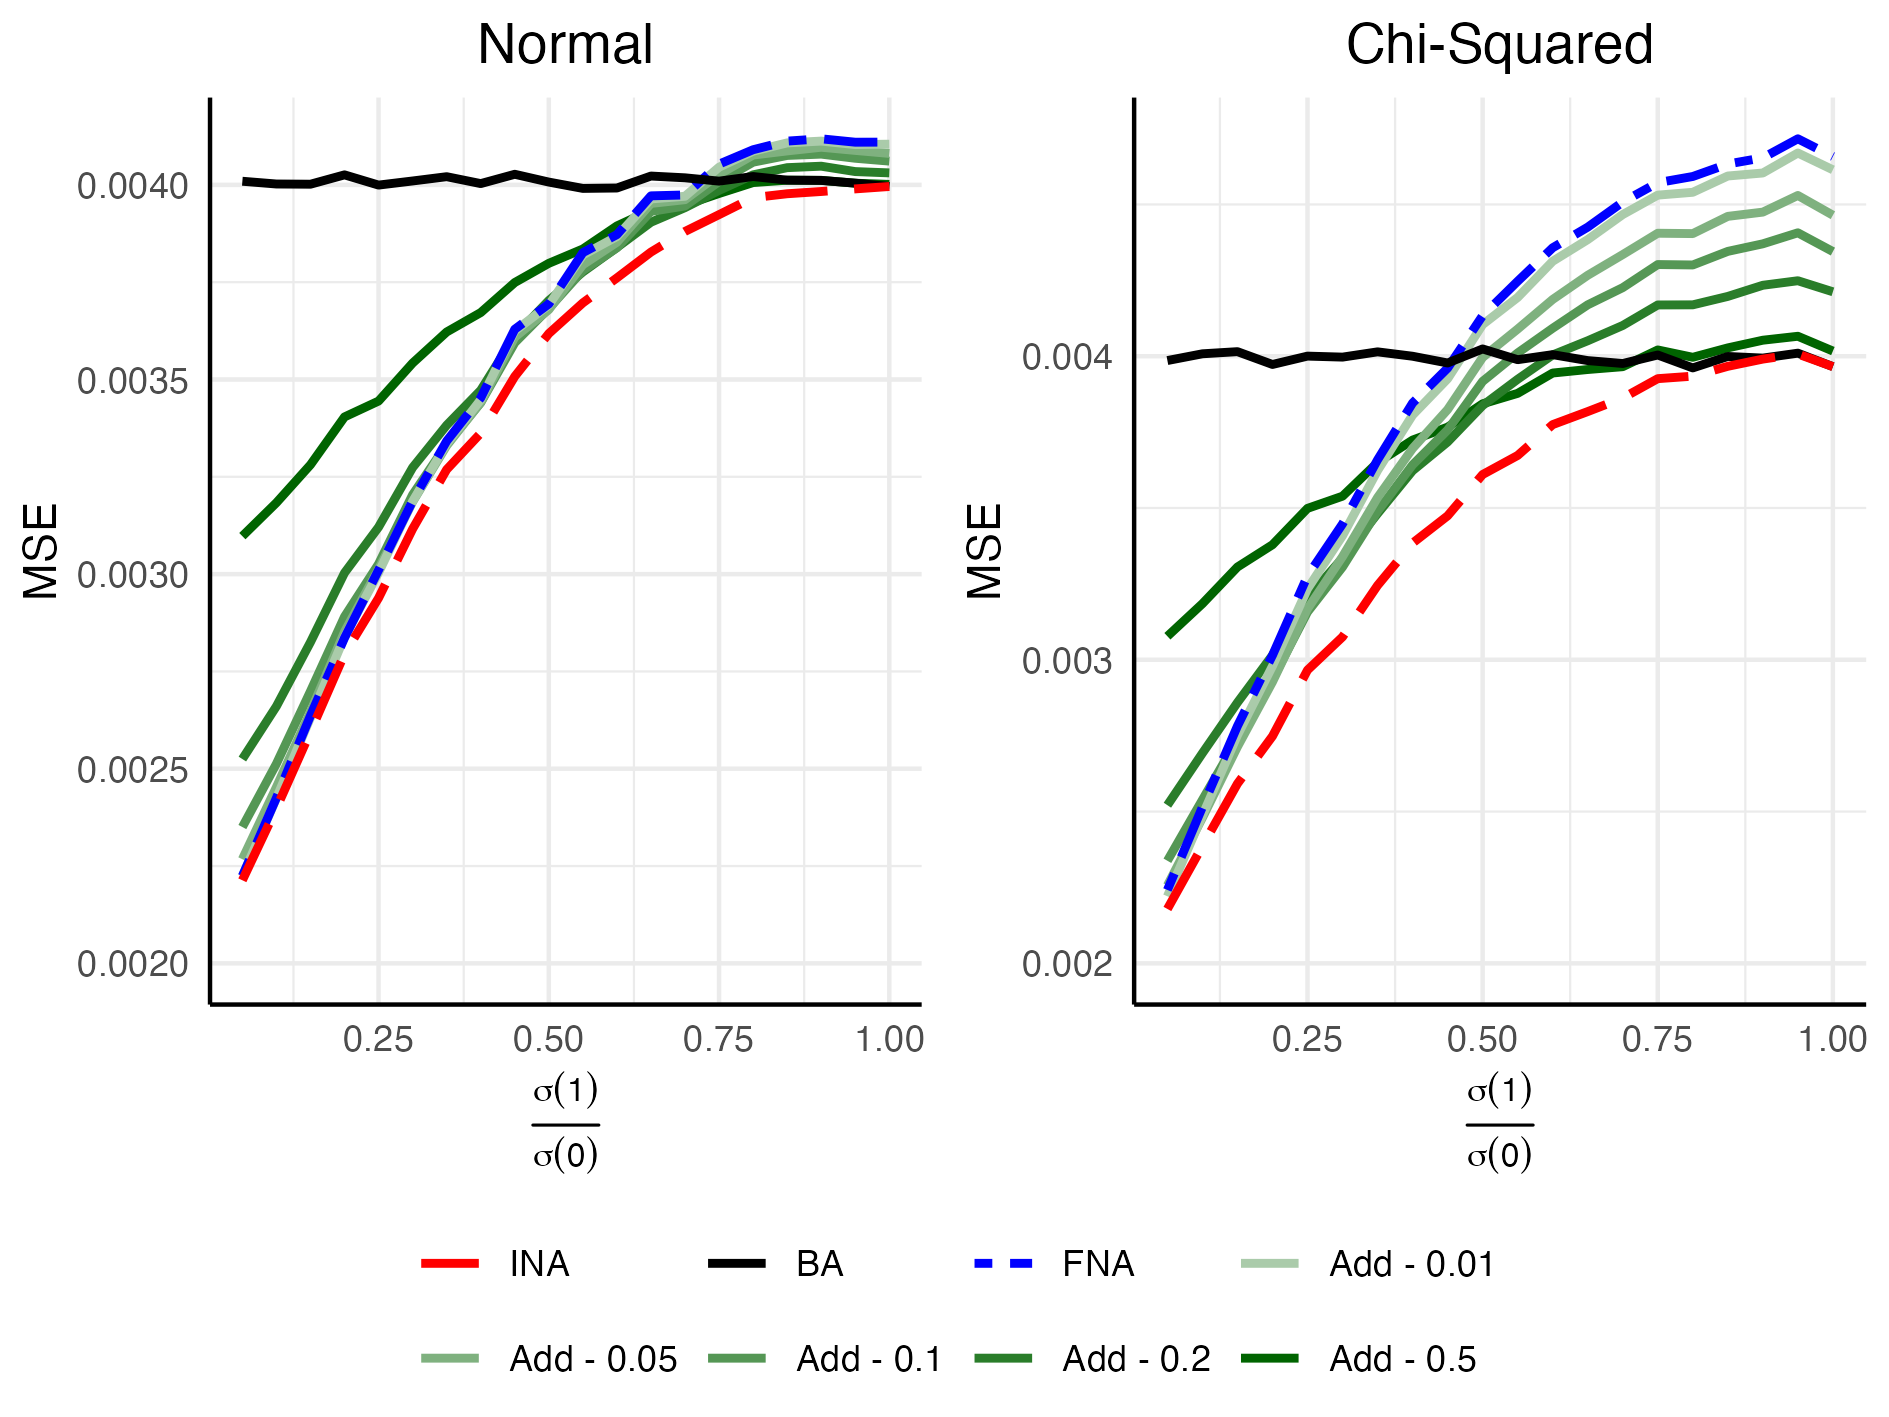
\includegraphics[width=\linewidth]{MSE_sol2_12}
%   \column{.5\linewidth}
%   \centering
%   Exponential (\(\tau\)) \\
%   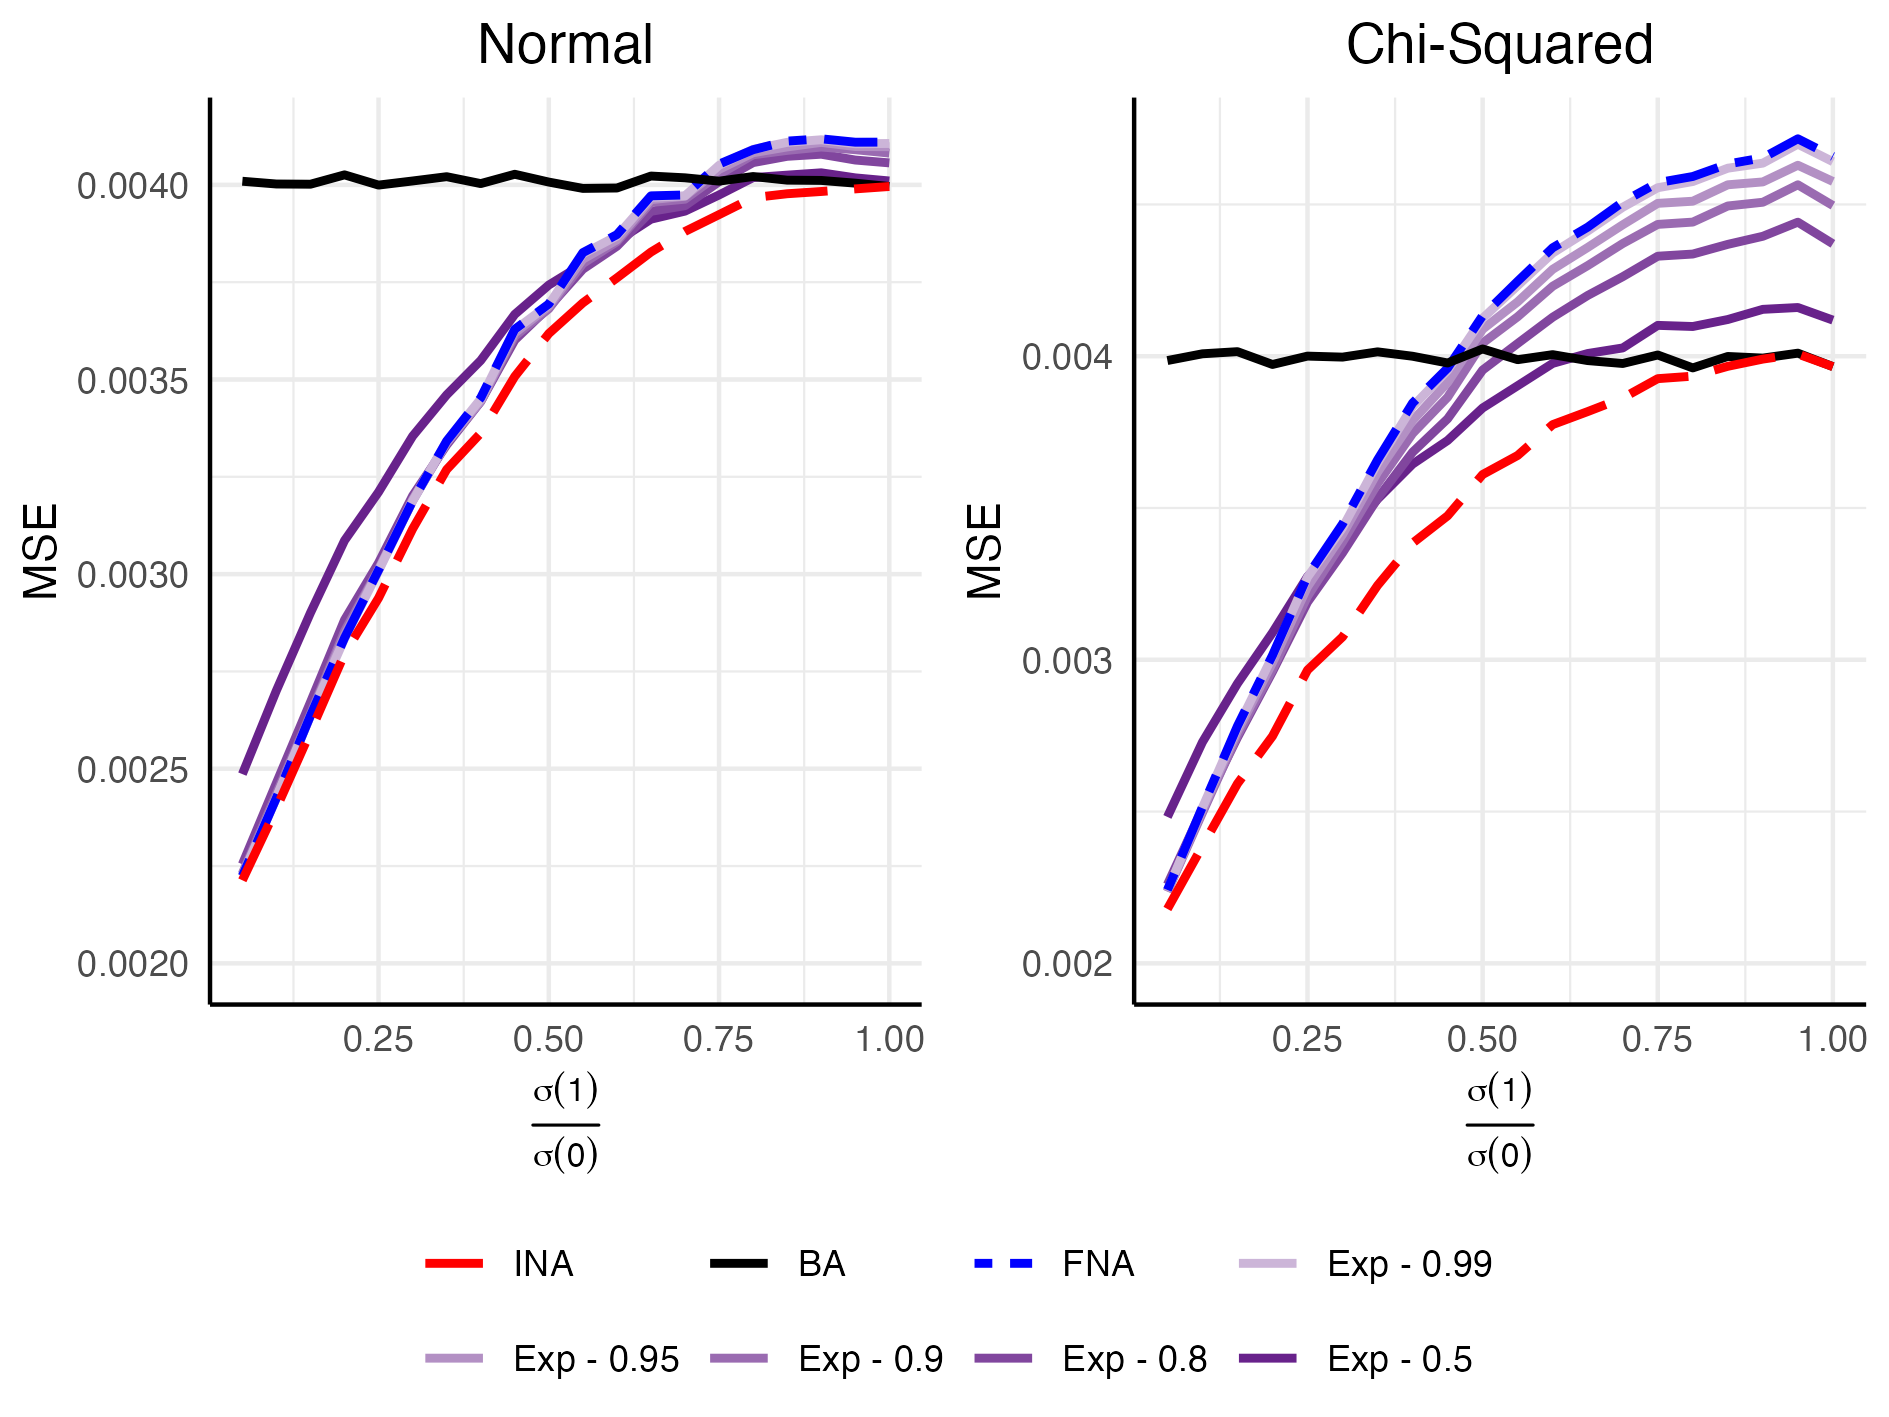
\includegraphics[width=\linewidth]{MSE_sol3_12}
% \end{columns}
% \vfill
% Both produce a continuum of trade-offs between homoskedastic and
% heteroskedastic regions.
% \end{frame}
%
% \begin{frame}
% \frametitle{Comparing the Three Solutions}
% \centering
% 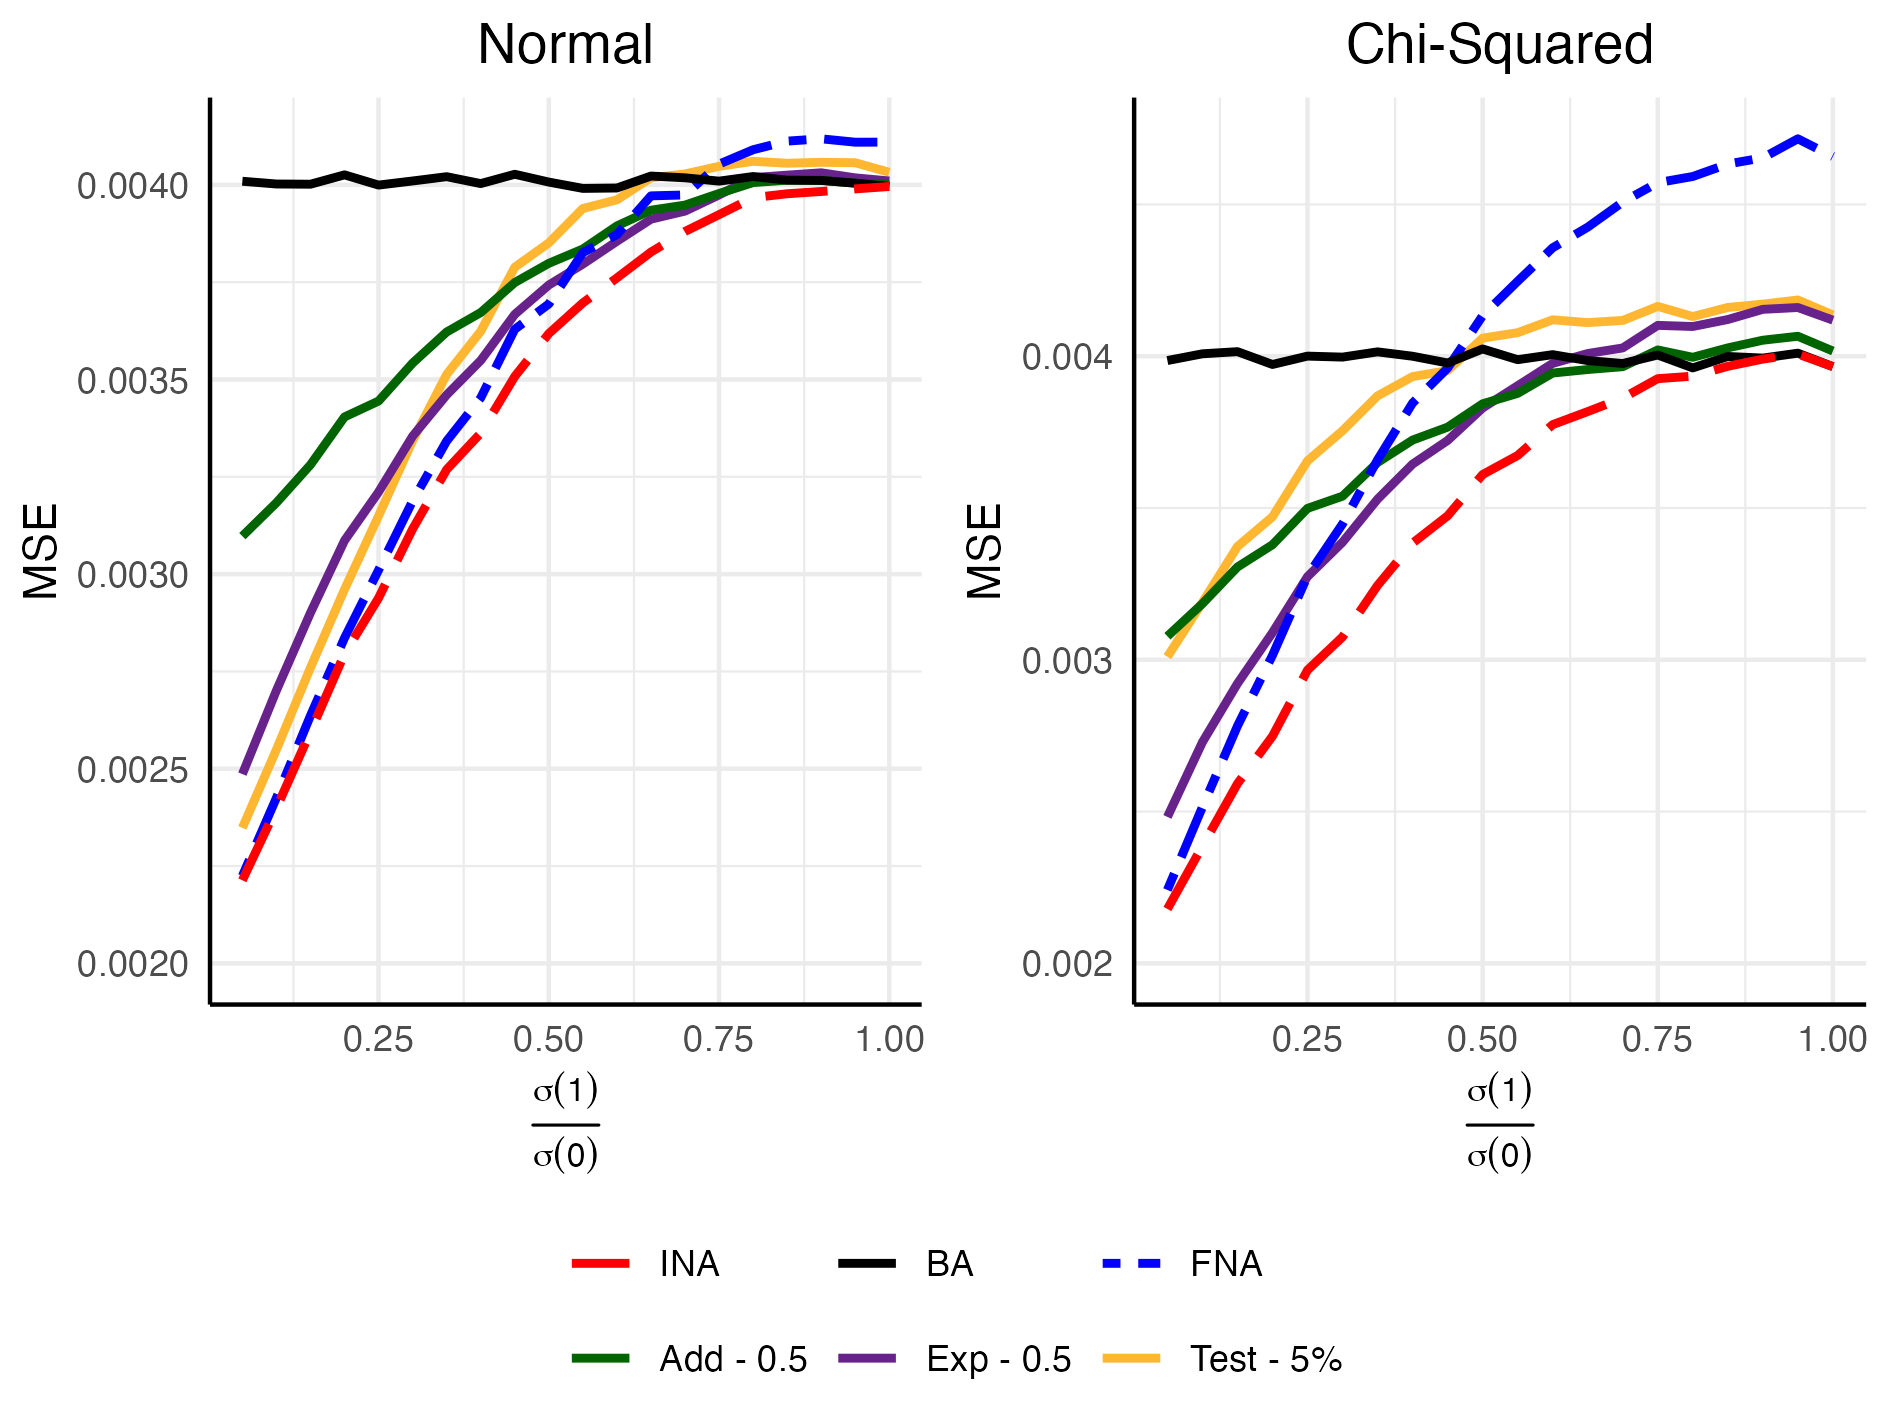
\includegraphics[width=.55\linewidth]{MSE_solcompare_12}
% \vfill
% \begin{itemize}
%   \item Tuning parameters chosen so MSE matches in the homoskedastic region.
%     \vfill
%   \item \textbf{Exponential regularization (yellow)} is uniformly best in
%     heteroskedastic region.
%     \vfill
%   \item Same conclusion holds for the Pareto DGPs (see appendix).
% \end{itemize}
% \end{frame}

%%%%%%%%%%%%%%%%%%%%%%%%%%%%%%%%%%%%%%%%%%%%%%%%%%%%%%%%%%%%%%%%%%%%%%%%%%%%%%%%
\section{Related literature and conclusion}
%%%%%%%%%%%%%%%%%%%%%%%%%%%%%%%%%%%%%%%%%%%%%%%%%%%%%%%%%%%%%%%%%%%%%%%%%%%%%%%%

\begin{frame}[plain,noframenumbering]
  \frametitle{Outline}
  \tableofcontents[currentsection]
\end{frame}

\begin{frame}
\frametitle{Recent related literature}
\begin{itemize}
  \item Optimal stratification in two-wave experiments:
    \citet{2023tabord-meehanStratificationTreesAdaptive,%
    2021cytrynbaumDesigningRepresentativeBalanced,%
    2023cytrynbaumOptimalStratificationSurvey,%
    2022baiOptimalityMatchedPair}.
    \vfill
  \item Batch-adaptive experiments: \citet{2023blackwellBatchAdaptiveDesigns}.
    \vfill
  \item Shrinkage-based adaptive allocation:
    \citet{2026rosenmanAdaptiveExperimentalDesign}
    \vfill
  \item This paper:
    \vfill
    \begin{itemize}
      \item Finite-pilot characterization of risks of feasible Neyman
        Allocation.
        \vfill
      \item Near-homoskedasticity and heavy tails.
        \vfill
      \item Regularized allocation rules --- simulation-based evidence, not in
        presentation.
    \end{itemize}
\end{itemize}
\end{frame}

\begin{frame}
\frametitle{Conclusion}
\begin{itemize}
  \item Use finite \(m\) to model statistical reality of most present two-wave
    experiments in social sciences.
    \vfill
  \item \textbf{Negative finding:} FNA can be strictly worse than 50/50
    randomization when outcomes are near-homoskedastic or heavy-tailed.
    \vfill
  \item Worst-case efficiency loss is \emph{unbounded}; worst-case gain is
    capped at \(1/2\).
    \vfill
  \item Empirical applications suggest bad cases happen fairly often.
    \vfill
  \item \textbf{Practical takeaway:} prefer BA under small pilots with near
    homoskedasticity or high kurtosis.
    \vfill
    \begin{itemize}
      \item Simulation-based result not in these slides: one can potentially use
        an exponentially regularized FNA --- seems to perform well even with
        near-homoskedasticity.
    \end{itemize}
\end{itemize}
\end{frame}

\begin{frame}[plain,noframenumbering]
\centering
\Large Thank you!
\end{frame}

%%%%%%%%%%%%%%%%%%%%%%%%%%%%%%%%%%%%%%%%%%%%%%%%%%%%%%%%%%%%%%%%%%%%%%%%%%%%%%%%
\section*{References}
%%%%%%%%%%%%%%%%%%%%%%%%%%%%%%%%%%%%%%%%%%%%%%%%%%%%%%%%%%%%%%%%%%%%%%%%%%%%%%%%

\begin{frame}[plain,noframenumbering,allowframebreaks]
\frametitle{References}
{\sloppy \printbibliography}
\end{frame}

%%%%%%%%%%%%%%%%%%%%%%%%%%%%%%%%%%%%%%%%%%%%%%%%%%%%%%%%%%%%%%%%%%%%%%%%%%%%%%%%
\section*{Appendix}
%%%%%%%%%%%%%%%%%%%%%%%%%%%%%%%%%%%%%%%%%%%%%%%%%%%%%%%%%%%%%%%%%%%%%%%%%%%%%%%%

\begin{frame}[t,plain,noframenumbering,allowframebreaks]
\frametitle{When is BA Better than FNA? PROOF
\hyperlink{frm--when-is-ba-better}{\beamergotobutton{RETURN}}}
\label{frm--prf--when-is-ba-better}
Denote \(x = \sigma (1) / \sigma (0)\), so that
\(\tilde{\pi}^{-1} = 1 + (x Z_{m})^{-1}\) and \((1 -
\tilde{\pi})^{-1} = 1 + x Z_{m}\).
Therefore, \(\Var_{\BA} \leq \Var_{\FNA}\) if and only if
\begin{equation*}
  \underbrace{\sigma^{2} (1) + \sigma^{2} (0)}_{= \sigma^{2} (0) (x^{2} + 1)}
  \leq \underbrace{\sigma^{2} (1) \E [(x Z_{m})^{-1}] +
  \sigma^{2} (0) x \E [Z_{m}]}_{= \sigma^{2} (0) (x^{2} \E [(x Z_{m})^{-1}] + x
  \E [Z_{m}])}.
\end{equation*}
So we want to find values of \(x = \sigma (1) / \sigma (0)\) for which
\(x^{2} - 2 B_{m} x + 1 \leq 0\).
\textbf{Solution set:}
\(x \in [c_{m, 1}, c_{m, 2}]\) where \(c_{m, j} = B_{m} + (- 1)^{j}
\sqrt{B_{m}^{2} - 1}\).

\hfill

\textbf{Note:} this is a real solution set since \(B_{m} \geq 1\) by the AM-GM
inequality: since both \(Z_{m}\) and \(Z_{m}^{- 1}\) are non-negative,
\(\frac{Z_{m}^{- 1} + Z_{m}}{2} \geq \sqrt{Z_{m}^{- 1} Z_{m}} = 1\).

\hfill

Now note that \(c_{m,1} = 1 / c_{m,2}\):
\begin{equation*}
  c_{m,1} c_{m,2} = (B_{m} - \sqrt{B_{m}^{2} - 1}) (B_{m} + \sqrt{B_{m}^{2} -
  1}) = B_{m}^{2} - (B_{m}^{2} - 1) = 1.
\end{equation*}
\end{frame}

\end{document}
